\chapter{Problemas de vibração livre com o método dos elementos virtuais}

\indent Neste capítulo, são analisados três problemas de vibração livre:

    \begin{itemize}
        \item Uma chapa engastada com furo circular no centro no estado plano de tensões;
        \item uma barragem de terra no estado plano de deformações, e
        \item uma parede estrutural de 4 pavimentos no estado plano de tensões. 
    \end{itemize}

\indent Todos os resultados aqui obtidos pelo MEV são comparados aos do MEF e aos do MEFG. Todas as três são técnicas numéricas que particionam o domínio em elementos e aproximam a solução localmente construindo sistemas de equações lineares. A principal diferença entre as técnicas é a maneira de construção da aproximação local.\\
\indent O MEF subdivide o espaço em elementos geométricos simples ou padronizados, como triângulos e retângulos. A aproximação da solução é feita unicamente com funções polinomiais, com a acurácia da solução dependendo do grau polinomial e da quantidade de elementos. Essa característica permite o mapeamento de todos os elementos através do uso de funções de forma, e a integração das matrizes de rigidez e massa pode ser feita diretamente através da quadratura de Gauss ou analiticamente para o caso de famílias de elementos não paramétricas. Porém, devido à limitação em relação aos tipos de elementos, a construção da malha deve ser rigorosa para não existir elementos muito distorcidos, com ângulos muito obtusos ou mal formados, pois estes degradam severamente a precisão da solução numérica.\\
\indent O MEFG é uma evolução do MEF utilizando a técnica de partição da unidade para enriquecer o espaço de aproximação. Enquanto a base do MEF é mantida, o MEFG multiplica as funções de forma por funções de enriquecimento que refletem o comportamento físico esperado do problema. Problemas abordados através do MEFG ganham graus de liberdade adicionais nos nós correspondentes aos modos de enriquecimento. As integrais são mais complexas e frequentemente exigem esquemas de integração numérica adaptativa ou mais refinados devido à aplicação de funções não polinomiais.\\
\indent Para a comparação dos resultados do MEV com resultados de referência obtidos pelo MEF e o MEFG desenvolvidos no capítulo 5 são
utilizadas as seguintes métricas
    \begin{enumerate}
        \item O erro médio absoluto (MAE)
        \item Erro percentual médio absoluto (MAPE) das frequências naturais para cada modo de vibração;
        \item Média da raiz erro ao quadrado normalizado (NRMSE)
        \item A média geométrica do erro (MG)
        \item Coeficiente de ácurácia de discretização (CAD)
        \item Ganho de precisão relativo (GPR)
        \item Capacidade de aproximação (CA)
    \end{enumerate}
    
\indent O erro relativo das frequências naturais para cada modo de vibração é calculado por:

\begin{equation}
    e_{rel} = \left| \frac{\omega - \tilde{\omega}}{\omega} \right|,
    \label{eq:1.1}
\end{equation}

\noindent com $\omega$ sendo a frequência de referência e $\tilde{\omega}$ a frequência obtida pelo MEV. Para a avaliação de um desempenho médio representativo dos dados utiliza-se a média do erro relativo percentual (MAPE), utilizado no trabalho de \citet{custodio2022metodo} e de \citet{torii2012analise} e sendo uma das médias mais comuns em diversos trabalhos. Para cada malha, a MAPE é medida pelo quociente entre a soma dos erros absolutos e a quantidade de modos analisados:	

\begin{equation}
    e_{MAPE} = \frac{\sum_{i=1}^{n_{modos}}e_{rel,i} }{n_{modos}}.
    \label{eq:1.2}
\end{equation}

\indent A média absoluta não pondera os resultados das frequências, de tal forma que um modo que possua um erro absoluto alto seja desconsiderado por outro modo com erro absoluto ótimo. Destarte, para estudo da eficiência global das malhas, será utilizado a raiz do erro quadrático médio (NRMSE):

\begin{equation}
    e_{NRMSE} = \sqrt{\frac{\sum_{i=1}^{n_{modos}} (\omega_i - \tilde{\omega}_i)^2}{\sum_{i=1}^{n_{modos}} (\omega_i)^2 }}. 
    \label{eq:1.3}
\end{equation}

\indent A NMRSE é uma métrica de erro baseada na norma $L^2$ representando a relação entre da "energia do erro" em relação a "energia global" da grandeza analisada. Por elevar os erros ao quadrado, o NRMSE garante uma penalização muito maior do que a do MAPE, o que o torna ideal para visualização dos resultados de maneira global.\\
\indent Tendo dois parâmetros de erro, propõem a utilização da média geométrica (MG) para unificação das médias dos erros como índice comparativo dos erros calculados como um índice composto:

\begin{equation}
    e_{MG} = \sqrt{e_{NRMSE} e_{MAPE} }.
    \label{eq:1.4}
\end{equation}

A escolha da média geométrica para índice composto é porque ela permite a união de dois parâmetros sem que um domine o outro.\\
\indent O coeficiente de acurácia de discretização (CAD) mede a evolução de uma malha conforme discretizada tomando como base a malha mais 
grossa, que possui menor custo computacional, para a malha mais refinada de maior custo. O parâmetro serve de indicativo para qual malha o 
refino $h$ atinge um teto de aproximação. O parâmetro é calculado por:

\begin{equation}
    CAD = \frac{\text{e}_{MG,\text{grossa}} - \text{e}_{MG,\text{atual}}}{\text{e}_{MG,\text{grossa}} - \text{e}_{MG,\text{refinada}}}.
    \label{eq:1.5}
\end{equation}

\indent Outra relação do CAD está relacionada ao ganho de acurácia em relação à malha mais grossa e de maneira inversa a malha mais refinada. 
Para o cálculo do CAD será utilizada a média geométrica como base.\\
\indent Visando à comparação entre métodos, um índice similar ao CAD é proposto, o ganho de precisão relativo (GPR). Esse índice mede a melhora de precisão entre dois métodos numéricos e um terceiro resultado de referência -- Numérico ou a solução exata. O índice é calculado como:

\begin{equation}
    GPR = \frac{\text{e}_{MG,\text{MEF}} - \text{e}_{MG,\text{MEV}}}{\text{e}_{MG,\text{MEF}}}.
    \label{eq:1.6}
\end{equation}

\indent O último parâmetro de estudo é baseado no índice CA elaborado por (\citet{cittadin2020enriquecimento}). Em seu uso original esse parâmetro mede as diferenças de
aproximação entre duas formulações com enriquecimento de funções e uma referência de base para estimativa de acurácia. O índice foi adaptado 
de modo que se possa comparar a diferença dos erros de duas técnicas numéricas em relação a uma terceira de referência. Este índice será 
utilizado neste trabalho para comparação do ganho de precisão entre o MEV e o MEFG em relação ao MEF clássico.

\begin{equation}
    CA = \frac{\text{e}_{MG,\text{MEF}} - \text{e}_{MG,\text{MEV}}}{\text{e}_{MG,\text{MEF}} - \text{e}_{MG,\text{MEFG}}}.
    \label{eq:1.7}
\end{equation}

\indent A avaliação dos resultados do CA segue:

\begin{enumerate}
    \item $CA < 0$: O MEV apresenta maior erro do que o MEF tradicional.
    \item $0 < CA < 1$: O MEV é mais preciso que o MEF, porém menos do que o MEFG.
    \item $CA = 1$: O MEV possui a mesma precisão do MEFG.
    \item $CA > 1$: O MEV supera tanto o MEF quanto o MEFG em precisão.
\end{enumerate}

\indent Neste trabalho a formulação do MEV e outras rotinas computacionais são implementadas com um solver programado em Modern Fortran
e o Gnuplot para visualização de resultados. Gráficos e tabelas comparativas são feitas com auxílio do Google planilhas. As malhas são gerados com o uso do software AutoCAD.\\[5mm]



\textbf{\underline{Esclarecimentos ao leitor:}}\\[2cm]

\indent Como os elementos virtuais podem possuir arestas com 180° entre si, podem existir malhas com a mesma quantidade de elementos, mas com diferentes quantidades de nós. Assim, adota-se o seguinte padrão de nomenclatura para as malhas utilizadas daqui em diante neste trabalho: $$XX+\#\#\#+N+\#\#\#+k\#$$. 

    \begin{itemize}
        \item X - Letras
        \item \# - Números
    \end{itemize}
    
\indent O primeiro conjunto de letras corresponde às iniciais do problema. O primeiro conjunto de números representa a quantidade de elementos na malha. N\#\#\# é a quantidade de nós. k\# é o grau polinomial que aqui varia de 1 a 2. Exemplo: PF32N74k1 $\rightarrow$ Placa com furo de 32 elementos, 74 nós e aproximação de primeira ordem. \\
\indent Todos os problemas aqui tratados são de natureza vetorial, assim a quantidade de graus de liberdade por elemento equivale a duas vezes a quantidade de nós. Em aproximações de segunda ordem, haverá dois graus de liberdade internos adicionais aos dos nós relativos a vetorização dos momentos internos para $k=2$. 

\section{Chapa com furo circular}

\indent O primeiro problema consiste em uma placa engastada de espessura unitária com um furo no centro, apresentando módulo de elasticidade $E = 1\text{ (N/m}^2\text{)}$, densidade constante no elemento $\rho = 1\text{ (kg/m}^3\text{)}$ e coeficiente de Poisson $\nu = 0,3$. A geometria pode ser observada na Figura~\ref{fig:5.1}.

    \begin{figure}[H]
        \centering
        \caption{Geometria e condições de contorno do problema da chapa com furo circular.}
        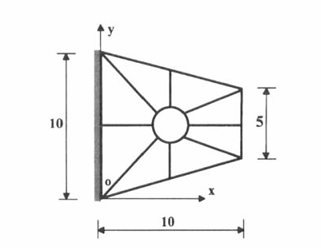
\includegraphics[width=\textwidth]{figuras/Capítulo 5/Placa com furo/5.1.png}
        \label{fig:5.1}
        {\small \textbf{Fonte:} \citet{asymptoticsolutionspredictednaturalfrequenciestwodimensionalelasticsolidvibrationproblemsfiniteelementanalysis1996}.}
    \end{figure}

\indent O problema foi proposto inicialmente no trabalho de \citet{asymptoticsolutionspredictednaturalfrequenciestwodimensionalelasticsolidvibrationproblemsfiniteelementanalysis1996} utilizando o estado plano de tensões. A intenção dos autores foi a utilização de correção dos resultados do método dos elementos finitos com o uso de soluções assintóticas, que, segundo eles, possui solução mais precisa. O mesmo problema foi abordado por \citet{cittadin2020enriquecimento} como referência de desempenho para o método dos elementos finitos generalizados. \\
\indent Para o problema da Figura~\ref{fig:5.1}, investiga-se o comportamento do método dos elementos virtuais para uma malha fixa de 8 elementos, contudo utilizando diferentes quantidades de nós na fronteira dos elementos com o furo para simular o contorno circular, Figura~\ref{fig:5.2}. 

    \begin{figure}[H]
        \centering
        \caption{Elementos de uma mesma malha com diferentes quantidades de nós. Observe que em a) o furo é modelado com apenas os dois nós de vértice e um nó interno, enquanto em b) há três nós internos modelando a geometria do furo. Estes nós foram adicionados sem alterar a ordem de interpolação polinomial.}
        \label{fig:5.2}
        \begin{subfigure}[b]{0.45\textwidth}
            \centering
            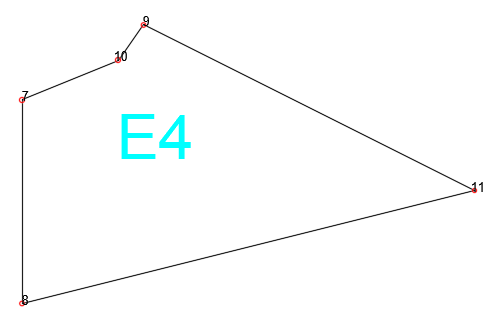
\includegraphics[width=\textwidth]{figuras/Capítulo 5/Placa com furo/f1.png}
            \label{fig:5.2a}
        \end{subfigure}
        \hfill
        \begin{subfigure}[b]{0.45\textwidth}
            \centering
            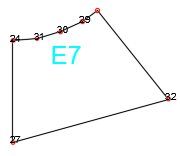
\includegraphics[width=\textwidth]{figuras/Capítulo 5/Placa com furo/f2.png}
            \label{fig:5.2b}
        \end{subfigure}
        \centerline{{\small \textbf{Fonte:} Elaborado pelo autor (2026).}}
    \end{figure}  

\indent Comparam-se os valores das frequências naturais em (rad/s) com as soluções analíticas -- obtidas de \citet{asymptoticsolutionspredictednaturalfrequenciestwodimensionalelasticsolidvibrationproblemsfiniteelementanalysis1996}, o modelo de elementos finitos de \citet{asymptoticsolutionspredictednaturalfrequenciestwodimensionalelasticsolidvibrationproblemsfiniteelementanalysis1996}, e o modelo de elementos finitos generalizados, com 480 graus de liberdade, de \citet{cittadin2020enriquecimento} para os primeiros dez modos de vibração. Os resultados se encontram resumidos na Tabela~\ref{tab:5.1}.


\begin{table}[H]
\caption{Frequências naturais obtidas para os primeiros dez modos de vibração (rad/s).}
\centering
\label{tab:5.1}
\begin{tabular}{llllrrrr}
\multirow{2}{*}{Modo} &
  \multicolumn{1}{c}{\multirow{2}{*}{\begin{tabular}[c]{@{}c@{}}REF\\ \citet{cittadin2020enriquecimento}\end{tabular}}} &
  \multicolumn{1}{c}{\begin{tabular}[c]{@{}c@{}}MEF\\ \citet{cittadin2020enriquecimento}\end{tabular}} &
  \multicolumn{1}{c}{\begin{tabular}[c]{@{}c@{}}MEFG\\ \citet{asymptoticsolutionspredictednaturalfrequenciestwodimensionalelasticsolidvibrationproblemsfiniteelementanalysis1996}\end{tabular}} &
  \multicolumn{4}{c}{VEM} \\
 &
  \multicolumn{1}{c}{} &
  32 gdl &
  480 gdl &
  \multicolumn{1}{c}{34 gdl} &
  \multicolumn{1}{c}{66 gdl} &
  \multicolumn{1}{c}{90 gdl} &
  \multicolumn{1}{c}{208 gdl} \\
1  & 0,0744 & 0,0833 & 0,0672 & 0,092 & 0,091 & 0,091 & 0,091 \\
2  & 0,1648 & 0,1661 & 0,1569 & 0,18  & 0,178 & 0,177 & 0,177 \\
3  & 0,2055 & 0,2334 & 0,1985 & 0,27  & 0,269 & 0,268 & 0,267 \\
4  & 0,2939 & 0,3302 & 0,2407 & 0,417 & 0,403 & 0,4   & 0,394 \\
5  & 0,3243 & 0,3525 & 0,2730 & 0,423 & 0,414 & 0,41  & 0,404 \\
6  & 0,4399 & 0,4234 & 0,3818 & 0,51  & 0,493 & 0,485 & 0,473 \\
7  & 0,4482 & 0,4624 & 0,4147 & 0,542 & 0,511 & 0,501 & 0,487 \\
8  & 0,4973 & 0,4805 & 0,4393 & 0,549 & 0,513 & 0,505 & 0,493 \\
9  & 0,5332 & 0,5508 & 0,4705 & 0,564 & 0,517 & 0,508 & 0,497 \\
10 & 0,5485 & 0,5578 & 0,5211 & 0,571 & 0,519 & 0,515 & 0,505 \\
\end{tabular}
\vspace{3mm}
{\small \textbf{Fonte:} Elaborado pelo autor (2026).}
\end{table}

\indent Observando os resultados da tabela, nota-se que os valores do método dos elementos virtuais se encontram acima tanto da solução assintótica quanto da de elementos finitos, o que leva a deduzir que existe uma adição de rigidez na formulação por conta do parâmetro de estabilização. Ao mesmo tempo, o método dos elementos finitos generalizados está no limite inferior da solução assintótica, levando a entender que existe um certo relaxamento da rigidez da formulação. \\
\indent Em uma pré-análise, calculam-se os erros relativos das malhas do método dos elementos virtuais tomando como referência a solução assintótica:

\begin{table}[H]
\caption{Erros relativos das malhas MEV em relação à solução assintótica de referência.}
\centering
\label{tab:5.2}
\begin{tabular}{rllll}
\multicolumn{1}{l}{MODO} & PF8N17k1 & PF8N33k1 & PF8N45k1 & PF8N104k1 \\
1                        & 23,66\%  & 22,31\%  & 22,31\%  & 22,31\%   \\
2                        & 9,22\%   & 8,01\%   & 7,40\%   & 7,40\%    \\
3                        & 31,39\%  & 30,90\%  & 30,41\%  & 29,93\%   \\
4                        & 41,88\%  & 37,12\%  & 36,10\%  & 34,06\%   \\
5                        & 30,43\%  & 27,66\%  & 26,43\%  & 24,58\%   \\
6                        & 15,94\%  & 12,07\%  & 10,25\%  & 7,52\%    \\
7                        & 20,93\%  & 14,01\%  & 11,78\%  & 8,66\%    \\
8                        & 10,40\%  & 3,16\%   & 1,55\%   & 0,86\%    \\
9                        & 5,78\%   & 3,04\%   & 4,73\%   & 6,79\%    \\
10                       & 4,10\%   & 5,38\%   & 6,11\%   & 7,93\%   
\end{tabular}
\centerline{{\small \textbf{Fonte:} Elaborado pelo autor (2026).}} 
\end{table}

\indent Como esperado, existe uma diminuição do erro conforme se aumenta a quantidade de graus de liberdade do sistema. Como notado por \citet{cittadin2020enriquecimento}, os erros na solução estão relacionados à geometria complexa do problema, sendo, assim, necessário um maior refino para que a solução convirja para a de referência. Propõem-se mais dois grupos de malhas: o primeiro grupo contendo 32 elementos e o segundo grupo com 64 elementos. Na Figura~\ref{fig:5.3a} a malha de 32 elementos possui 62, 82 e 103 nós respectivamente. Para a malha da Figura~\ref{fig:5.3b} com 64 elementos utiliza-se 105 e 114 nós. A Tabela~\ref{tab:5.3} apresenta as frequências obtidas para essas duas malhas.

    \begin{figure}[H]
        \centering
        \caption{Malhas de 32 e 64 elementos}
        \label{fig:5.3}
        \begin{subfigure}[b]{0.45\textwidth}
            \centering
            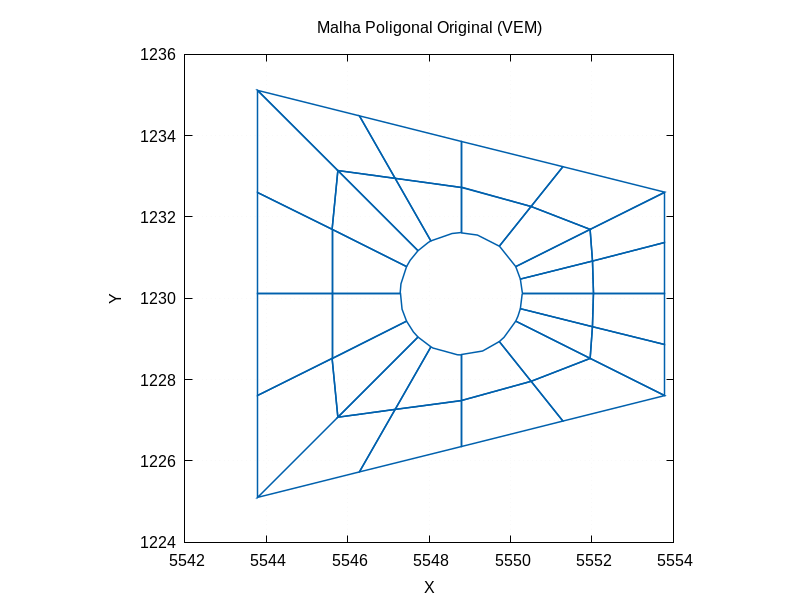
\includegraphics[width=\textwidth]{figuras/Capítulo 5/Placa com furo/malha não deformada 32.png}
            \label{fig:5.3a}
        \end{subfigure}
        \hfill
        \begin{subfigure}[b]{0.45\textwidth}
            \centering
            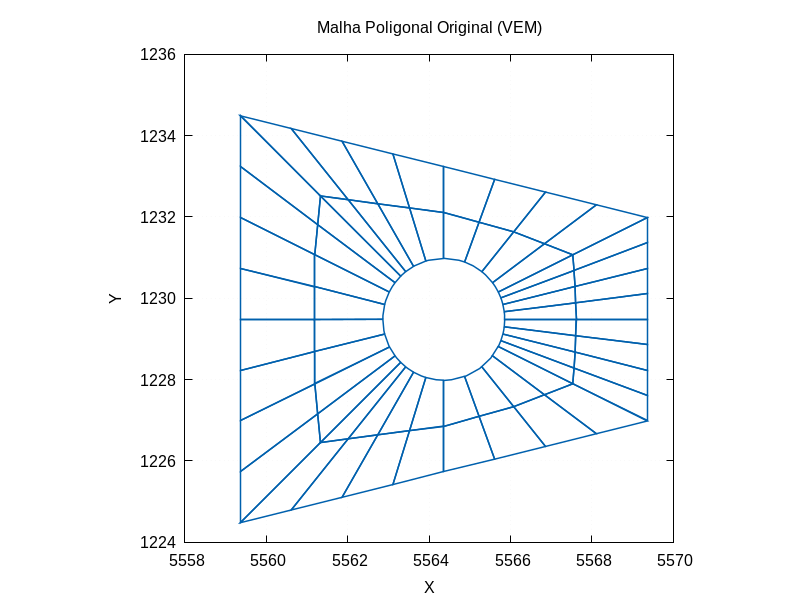
\includegraphics[width=\textwidth]{figuras/Capítulo 5/Placa com furo/mallha não deformada 64.png}
            \label{fig:5.3b}
        \end{subfigure}
        \centerline{{\small \textbf{Fonte:} Elaborado pelo autor (2026).}}
    \end{figure}  

\begin{table}[H]
\caption{Erros relativos das frequências para as malhas de 32 e 64 elementos.}
\centering
\label{tab:5.3}
\begin{tabular}{rlllll}
\multicolumn{1}{l}{MODO} & PF32N62k1 & PF32N82k1 & PF32N103k1 & PF64N105k1 & PF64N114k1 \\
1                        & 12,90\%   & 12,90\%   & 12,90\%    & 19,35\%    & 24,73\%    \\
2                        & 3,76\%    & 3,76\%    & 2,55\%     & 56,31\%    & 49,64\%    \\
3                        & 14,36\%   & 14,36\%   & 14,36\%    & 63,02\%    & 33,82\%    \\
4                        & 24,19\%   & 23,85\%   & 21,13\%    & 58,15\%    & 40,46\%    \\
5                        & 18,72\%   & 18,10\%   & 17,79\%    & 48,81\%    & 38,33\%    \\
6                        & 10,71\%   & 10,71\%   & 7,98\%     & 51,58\%    & 50,44\%    \\
7                        & 20,71\%   & 20,71\%   & 19,59\%    & 40,87\%    & 21,02\%    \\
8                        & 9,99\%    & 9,99\%    & 9,19\%     & 29,82\%    & 20,17\%    \\
9                        & 18,90\%   & 17,22\%   & 17,40\%    & 25,92\%    & 21,61\%    \\
10                       & 22,88\%   & 22,33\%   & 19,23\%    & 25,43\%    & 21,60\%   
\end{tabular}
\centerline{{\small \textbf{Fonte:} Elaborado pelo autor (2026).}}
\end{table}

\begin{figure}[H]
    \centering
    \caption{Comparação das frequências obtidas por modo de vibração para a placa engastada com furo.}
    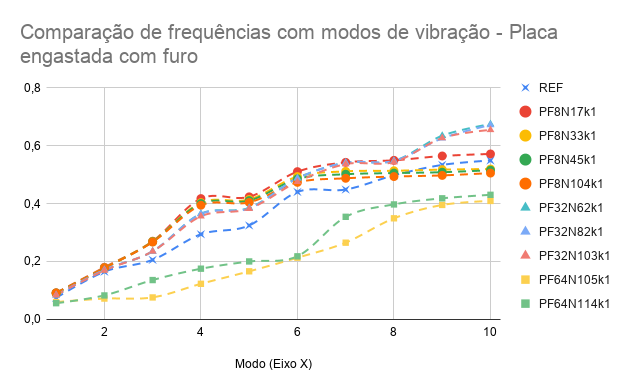
\includegraphics[width=\textwidth]{figuras/Capítulo 5/Placa com furo/Comparação de frequências com modos de vibração - Placa engastada com furo.png}
    \label{fig:5.4}
    \centerline{    {\small \textbf{Fonte:} Elaborado pelo autor (2026).}}

\end{figure}

\indent Percebe-se para a malha de 32 elementos uma leve aproximação da solução de referência quando comparada à malha de 8 elementos para os primeiros modos. Contudo, a partir do quarto modo, existe um aumento no valor das frequências em comparação com a malha de 8 elementos. Para a malha de 64 elementos, observa-se uma inversão logo nos primeiros modos, em que a frequência se torna menor que a referência e mantém-se assim para todos os modos subsequentes. Investigando o fenômeno mais a fundo, calcularam-se os erros relativos de cada frequência, sumarizados na Tabela~\ref{tab:5.4} e ilustrados na Figura~\ref{fig:5.4}.

\begin{table}[H]
\caption{Resumo dos erros relativos de frequência (\%) para todas as malhas analisadas.}
\centering
\label{tab:5.4}
\begin{tabular}{rlllllllll}
\multicolumn{1}{l}{MODO} & PF8N17k1 & PF8N33k1 & PF8N45k1 & PF8N104k1 & PF32N62k1 & PF32N82k1 & PF32N103k1 & PF64N105k1 & PF64N114k1 \\
1  & 23,66\% & 22,31\% & 22,31\% & 22,31\% & 12,90\% & 12,90\% & 12,90\% & 19,35\% & 24,73\% \\
2  & 9,22\%  & 8,01\%  & 7,40\%  & 7,40\%  & 3,76\%  & 3,76\%  & 2,55\%  & 56,31\% & 49,64\% \\
3  & 31,39\% & 30,90\% & 30,41\% & 29,93\% & 14,36\% & 14,36\% & 14,36\% & 63,02\% & 33,82\% \\
4  & 41,88\% & 37,12\% & 36,10\% & 34,06\% & 24,19\% & 23,85\% & 21,13\% & 58,15\% & 40,46\% \\
5  & 30,43\% & 27,66\% & 26,43\% & 24,58\% & 18,72\% & 18,10\% & 17,79\% & 48,81\% & 38,33\% \\
6  & 15,94\% & 12,07\% & 10,25\% & 7,52\%  & 10,71\% & 10,71\% & 7,98\%  & 51,58\% & 50,44\% \\
7  & 20,93\% & 14,01\% & 11,78\% & 8,66\%  & 20,71\% & 20,71\% & 19,59\% & 40,87\% & 21,02\% \\
8  & 10,40\% & 3,16\%  & 1,55\%  & 0,86\%  & 9,99\%  & 9,99\%  & 9,19\%  & 29,82\% & 20,17\% \\
9  & 5,78\%  & 3,04\%  & 4,73\%  & 6,79\%  & 18,90\% & 17,22\% & 17,40\% & 25,92\% & 21,61\% \\
10 & 4,10\%  & 5,38\%  & 6,11\%  & 7,93\%  & 22,88\% & 22,33\% & 19,23\% & 25,43\% & 21,60\%
\end{tabular}
\centerline{{\small \textbf{Fonte:} Elaborado pelo autor (2026).}}

\end{table}

\indent Da Figura~\ref{fig:5.4}, constatam-se as observações feitas na tabela: 

\begin{itemize}
    \item As malhas de 32 elementos apresentam frequências similares às de referência apenas para os primeiros modos de vibração.
    \item A malha com 64 elementos apresenta valores muito inferiores aos de referência, mesmo com o aumento da quantidade de graus de liberdade.
    \item As curvas variam entre si conforme a quantidade de elementos, mas a variação das frequências de malhas com a mesma quantidade de elementos apresenta pouca variação entre si.
\end{itemize}

\indent Para compreender o fenômeno que ocorre nas malhas de 64 elementos, analisa-se o condicionamento da matriz de rigidez:

\begin{table}[H]
\caption{Número de condicionamento da matriz de rigidez $K_{ii}$ para cada malha.}
\label{tab:5.5}
\begin{tabular}{lllr}
Configuração & Elementos & GDL & \multicolumn{1}{l}{Condicionamento de $K_{ii}$} \\
PF8N17k1     & 8         & 34  & 2,16E+02                                      \\
PF8N33k1     & 8         & 66  & 3,40E+02                                      \\
PF8N45k1     & 8         & 90  & 4,55E+02                                      \\
PF8N104k1    & 8         & 208 & 1,07E+03                                      \\
PF32N62k1    & 32        & 124 & 1,47E+03                                      \\
PF32N82k1    & 32        & 164 & 1,87E+03                                      \\
PF32N103k1   & 32        & 206 & 2,29E+03                                      \\
PF64N105k1   & 64        & 210 & 6,94E+04                                      \\
PF64N114k1   & 64        & 228 & 3,39E+04                                     
\end{tabular}
\centerline{{\small \textbf{Fonte:} Elaborado pelo autor (2026).}}

\end{table}

\begin{figure}[H]
    \centering
    \caption{Condicionamento de $K$ em função das malhas utilizadas.}
    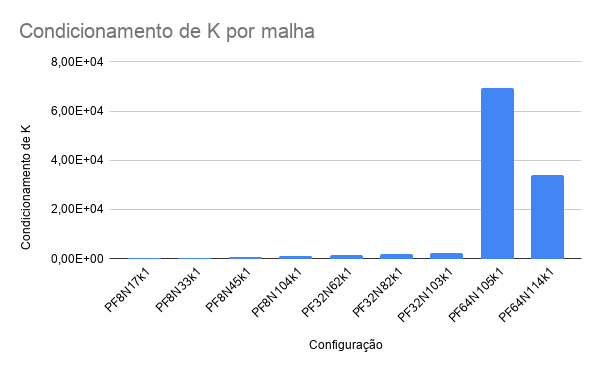
\includegraphics[width=\textwidth]{figuras/Capítulo 5/Placa com furo/Condicionamento de K por malha.png}
    \label{fig:5.5}
    \centerline{    {\small \textbf{Fonte:} Elaborado pelo autor (2026).}}

\end{figure}

\indent Observa-se na Figura~\ref{fig:5.5} que o valor do condicionamento da matriz de rigidez para a primeira malha assume valores maiores que $6 \times 10^4$. Como destacado por \citet{stabilityanalysisvirtualelementmethod2016a}, polígonos com arestas muito menores que o diâmetro dos elementos comprometem a coercividade da constante de estabilidade, e \citet{illconditioningvirtualelementmethodstabilizationsbases2018} demonstra que polígonos malformados comprometem o condicionamento. A grande quantidade de elementos na malha mais refinada faz com que os elementos que fazem fronteira com o furo possuam arestas muito pequenas, prejudicando a estabilidade do método.\\
\indent Buscando validar os resultados, foram calculados os erros MAPE, NRMSE e MG para cada uma das malhas. Os resultados estão resumidos na Tabela~\ref{tab:5.6} e a curva entre os erros é apresentada na Figura~\ref{fig:5.6}:

\begin{figure}[H]
    \centering
    \caption{Curva de erros para a placa engastada com furo.}
    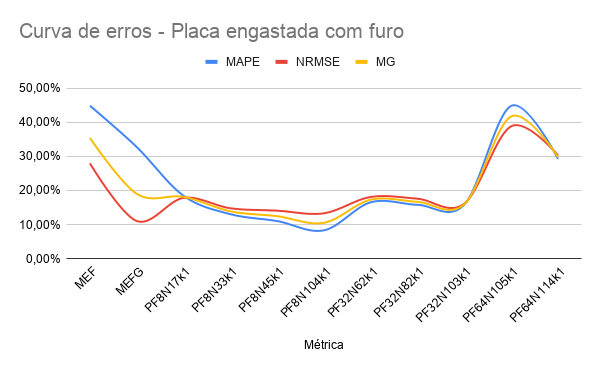
\includegraphics[width=\textwidth]{figuras/Capítulo 5/Placa com furo/Curva de erros - Placa engastada com furo.png}
    \label{fig:5.6}
    \centerline{    {\small \textbf{Fonte:} Elaborado pelo autor (2026).}}

\end{figure}


\begin{table}[H]
\caption{Métricas de erro global (MAPE, NRMSE e MG) para cada malha da placa engastada.}
\label{tab:5.6}
\begin{tabular}{llllllllll}
\textbf{Métrica} & PF8N17k1 & PF8N33k1 & PF8N45k1 & PF8N104k1 & PF32N62k1 & PF32N82k1 & PF32N103k1 & PF64N105k1 & PF64N114k1 \\
MAPE  & 18,43\% & 13,04\% & 11,02\% & 8,29\%  & 16,54\% & 15,79\% & 15,88\% & 44,84\% & 29,28\% \\
NRMSE & 17,82\% & 14,77\% & 14,07\% & 13,30\% & 18,11\% & 17,57\% & 16,15\% & 38,86\% & 30,28\% \\
MG    & 18,12\% & 13,88\% & 12,45\% & 10,50\% & 17,30\% & 16,65\% & 16,01\% & 41,74\% & 29,77\%
\end{tabular}
\centerline{{\small \textbf{Fonte:} Elaborado pelo autor (2026).}}

\end{table}

\begin{figure}[H]
    \centering
    \caption{Coeficiente de acurácia global para as malhas da placa engastada.}
    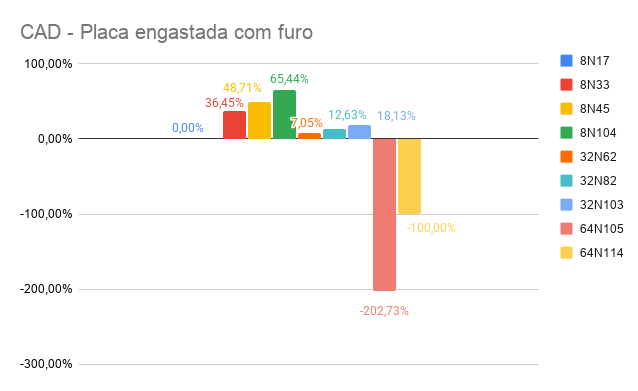
\includegraphics[width=\textwidth]{figuras/Capítulo 5/Placa com furo/CAD - Placa engastada com furo.png}
    \label{fig:5.7}
    \centerline{    {\small \textbf{Fonte:} Elaborado pelo autor (2026).}}

\end{figure}


\indent Analisando os erros, é curioso notar que a malha com menor erro é a de 8 elementos com 104 nós, e não a de 32 elementos. Beirão da Veiga et al. \citet{basicprinciplesvirtualelementmethods2013a} comentam que o Método dos Elementos Virtuais apresenta a capacidade de lidar com elementos contendo quantidades arbitrárias de nós e formatos complexos, evitando a rigidez artificial imposta pelo particionamento do domínio em elementos padrões.\\
\indent O termo $\Lambda$, utilizado para penalização no termo de estabilidade deste trabalho, emprega o traço da matriz de rigidez consistente como constante multiplicativa. Como explicado por \citet{basicformulationsvirtualelementmethodvemfinitedeformations2017}, essa escolha evita o travamento volumétrico e aumenta a robustez computacional para sólidos submetidos a grandes deformações, fazendo com que o termo de estabilização escale na mesma ordem de grandeza da matriz de consistência.\\
\indent Conforme destacado em \citet{illconditioningvirtualelementmethodstabilizationsbases2018}, o espaço de solução local pode ser particionado em uma componente polinomial e outra puramente virtual:

\begin{equation}
    \begin{aligned}
        V_k (\Omega) = \left\{ v_k \in V_k(\Omega) \mid v_k \in \mathbb{P}_k(\Omega) \right\} \oplus \left\{ v_k \in V_k(\Omega) \mid \Pi_k^\nabla v_k = 0 \right\}\\ = \mathbb{P}_k(\Omega) \oplus \ker(\Pi^\nabla_k) = V_{k,1} \oplus V_{k,2}
    \end{aligned}
\end{equation}

de tal modo que uma função polinomial seja nula no espaço puramente virtual $V_{k,2}$ e uma função virtual se anule no espaço polinomial $V_{k,1}$. Próximo à região do furo, os campos de deformação apresentam elevados gradientes, fazendo com que a projeção polinomial não capture toda a cinemática local e resultando em uma contribuição significativa da componente puramente virtual (e, consequentemente, da matriz de estabilização).\\
\indent Como notado por Mora et al. \citet{virtualelementmethodstekloveigenvalueproblemallowingsmalledges2020a}, o parâmetro de estabilização pode afetar a aproximação do espectro de autovalores, resultando em um problema discreto excessivamente rígido e poluindo severamente as frequências mais altas, particularmente quando malhas distorcidas são empregadas. Assim, com o aumento da quantidade de elementos na região do furo, há também o aumento do número de matrizes de estabilização locais somadas ao sistema, impondo uma rigidez artificial global à solução que degrada os resultados da malha de 32 elementos.
Outro detalhe que pode ser visto analisando os resultados da Tabela~\ref{tab:5.4} é a malha de 8 elementos possuir maiores erros em relação aos primeiros modos de vibração quando comparada à malha de 32 elementos. Isso demonstra que o refino de uma malha de 32 seria o ideal se não fossem os erros acumulados da estabilização. Com essa consideração, trabalhos futuros podem realizar essa mesma análise utilizando a formulação livre de estabilização do método dos elementos virtuais e comparar os resultados.\\
\indent Assim como descrito no capítulo 3, na análise modal cada modo apresenta uma resposta harmônica no tempo, apesar das diferentes amplitudes. Essa propriedade é ilustrada na Figura~\ref{fig:5.8}.

\begin{figure}[H]
    \centering
    \caption{Malha de 8 elementos deformada com aumento da quantidade de graus de liberdade na fronteira com o furo.}
    \label{fig:5.8}
    \begin{subfigure}[b]{0.45\textwidth}
        \centering
        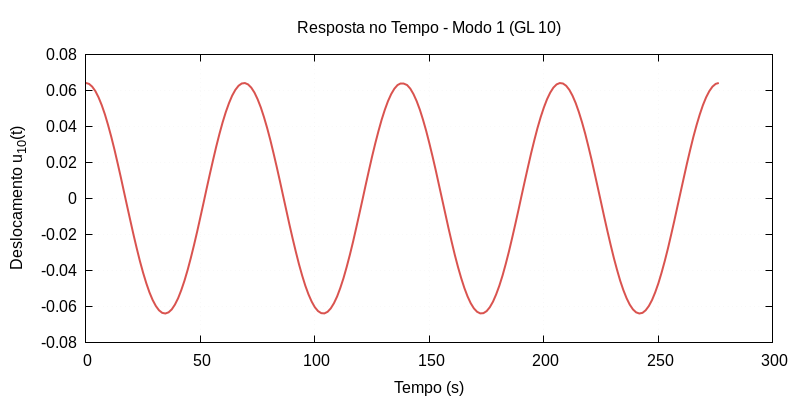
\includegraphics[width=\textwidth]{figuras/Capítulo 5/Placa com furo/time_disp_mode_1_dof_10.png}
        \label{fig:5.8a}
    \end{subfigure}
    \hfill
    \begin{subfigure}[b]{0.45\textwidth}
        \centering
        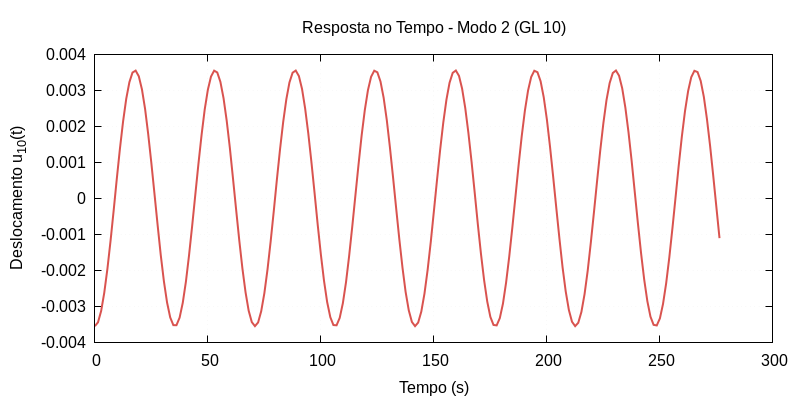
\includegraphics[width=\textwidth]{figuras/Capítulo 5/Placa com furo/time_disp_mode_2_dof_10.png}
        \label{fig:5.8b}
    \end{subfigure}
    \vspace{3mm}
    \begin{subfigure}[b]{0.45\textwidth}
        \centering
        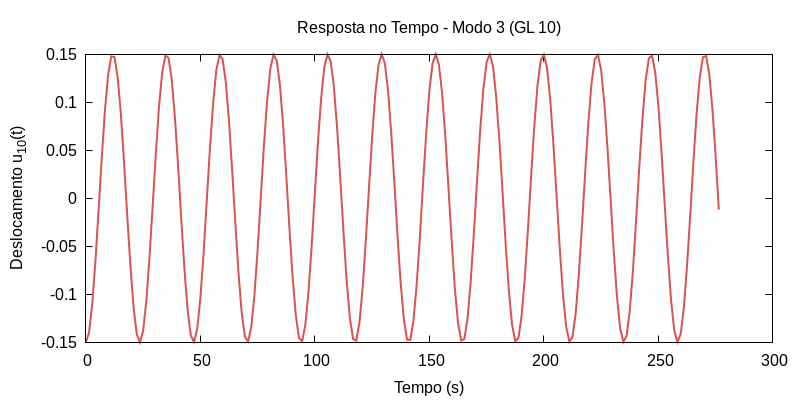
\includegraphics[width=\textwidth]{figuras/Capítulo 5/Placa com furo/time_disp_mode_3_dof_10.png}
        \label{fig:5.8c}
    \end{subfigure}
    \hfill
    \begin{subfigure}[b]{0.45\textwidth}
        \centering
        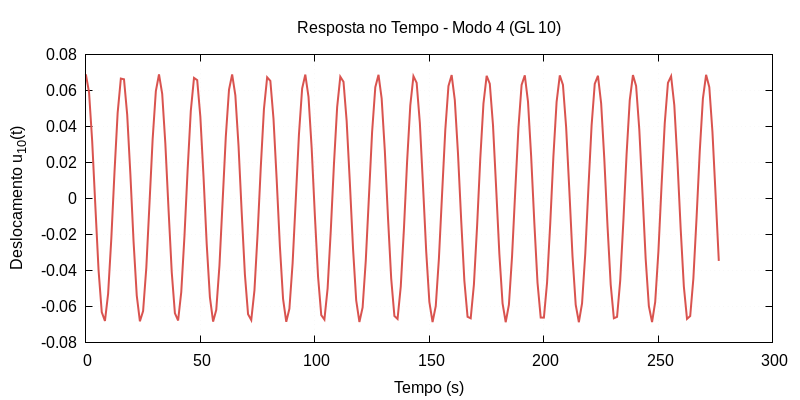
\includegraphics[width=\textwidth]{figuras/Capítulo 5/Placa com furo/time_disp_mode_4_dof_10.png}
        \label{fig:5.8d}
    \end{subfigure}
    \centerline{    {\small \textbf{Fonte:} Elaborado pelo autor (2026).}}

\end{figure}  

\begin{figure}[H]
    \centering
    \caption{Deformação do 10º modo de vibração para diferentes refinos de nós na malha de 8 elementos.}
    \label{fig:5.9}
    \begin{subfigure}[b]{0.45\textwidth}
        \centering
        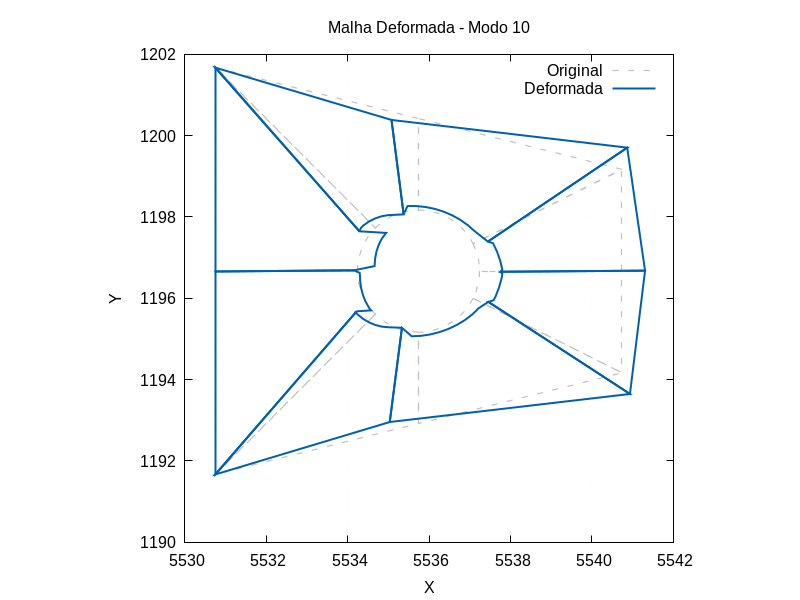
\includegraphics[width=\textwidth]{figuras/Capítulo 5/Placa com furo/Malha 8-104 deformação do modo 10.png}
        \label{fig:5.9a}
    \end{subfigure}
    \hfill
    \begin{subfigure}[b]{0.45\textwidth}
        \centering
        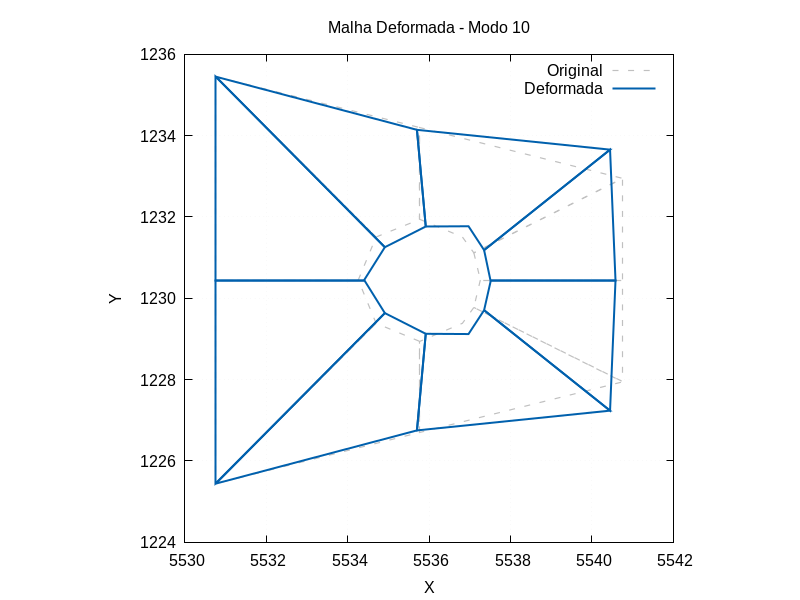
\includegraphics[width=\textwidth]{figuras/Capítulo 5/Placa com furo/Malha 8-17 deformação do modo 10.png}
        \label{fig:5.9b}
    \end{subfigure}
    \vspace{3mm}
    \begin{subfigure}[b]{0.45\textwidth}
        \centering
        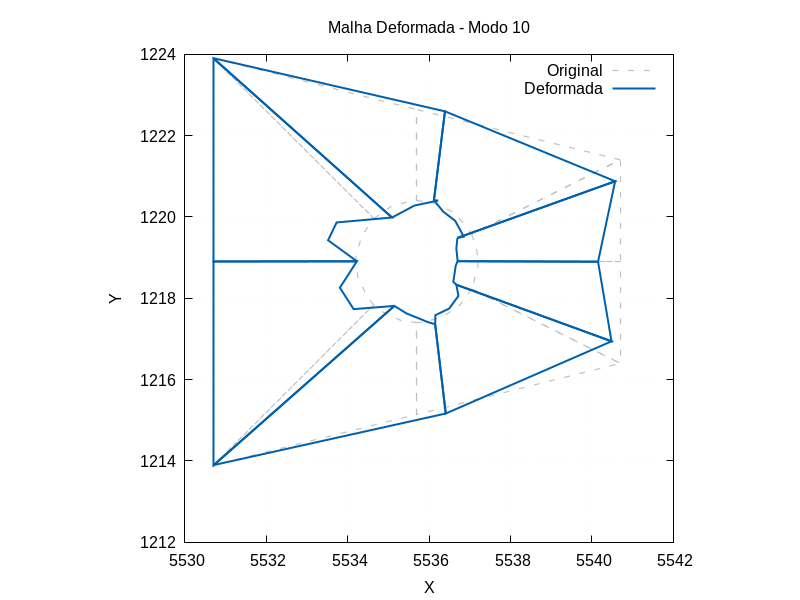
\includegraphics[width=\textwidth]{figuras/Capítulo 5/Placa com furo/Malha 8-33 deformação do modo 10.png}
        \label{fig:5.9c}
    \end{subfigure}
    \hfill
    \begin{subfigure}[b]{0.45\textwidth}
        \centering
        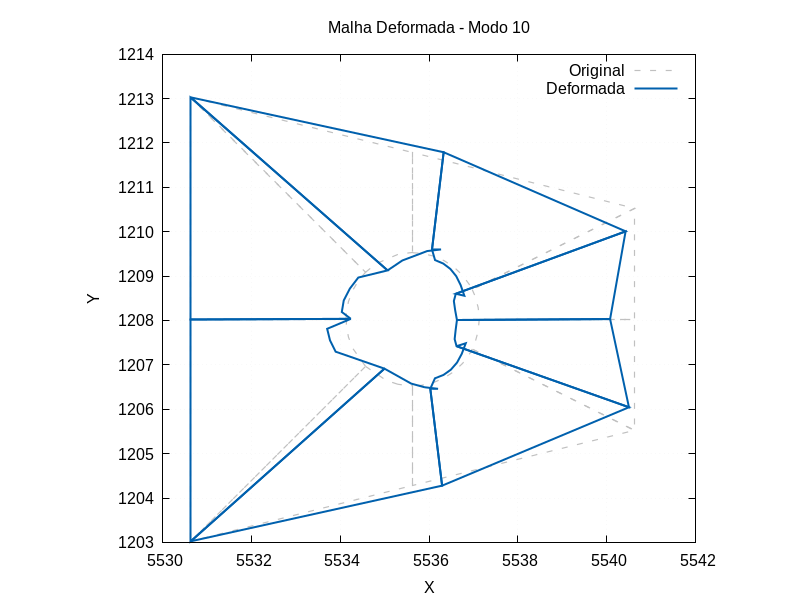
\includegraphics[width=\textwidth]{figuras/Capítulo 5/Placa com furo/Malha 8-45 deformação do modo 10.png}
        \label{fig:5.9d}
    \end{subfigure}
    \centerline{    {\small \textbf{Fonte:} Elaborado pelo autor (2026).}}

\end{figure}  

\indent O estudo do ganho de precisão relativo do método foi executado para a formulação de elementos finitos clássica apresentada no trabalho de \citet{asymptoticsolutionspredictednaturalfrequenciestwodimensionalelasticsolidvibrationproblemsfiniteelementanalysis1996} -- e não a versão com correção.

\begin{table}[H]
\caption{Ganho de precisão relativo no problema da placa engastada com furo.}
\label{tab:5.7}
\begin{tabular}{l *{10}{>{\centering\arraybackslash}p{1.2cm}}}
\textbf{Métrica} &
\textbf{MEF (REF)} & 
\textbf{PF8 N17 k1} & 
\textbf{PF8 N33 k1} & 
\textbf{PF8 N45 k1} & 
\textbf{PF8 N104 k1} & 
\textbf{PF32 N62 k1} & 
\textbf{PF32 N82 k1} & 
\textbf{PF32 N103 k1} & 
\textbf{PF64 N105 k1} & 
\textbf{PF64 N114 k1} \\
\hline
MAPE  & 38,80\% & 52\%   & 66\%   & 72\%   & 79\%   & 57\%   & 59\%   & 59\%   & -16\%  & 25\%   \\
NRMSE & 5,26\%  & -239\% & -181\% & -168\% & -153\% & -245\% & -234\% & -207\% & -639\% & -476\% \\
MG    & 14,28\% & -27\%  & 3\%    & 13\%   & 26\%   & -21\%  & -17\%  & -12\%  & -192\% & -109\%
\end{tabular}
\vspace{2mm}
\centerline{\small \textbf{Fonte:} Elaborado pelo autor (2026).}
\end{table}

\indent Através do cálculo do GPR, observa-se que a malha de 34 graus de liberdade, que possui apenas dois graus de liberdade a mais que a malha de \citet{asymptoticsolutionspredictednaturalfrequenciestwodimensionalelasticsolidvibrationproblemsfiniteelementanalysis1996}, apresenta perda na precisão de 27\% para malhas irregulares e desestruturadas. O ganho de precisão se inicia a partir da malha de 66 graus de liberdade com 3\% e sobe para 26\% com o acréscimo de até 174 graus de liberdade para modelar o furo.\\
\indent Para o estudo da acurácia entre o método dos elementos finitos generalizados e o método dos elementos virtuais, utilizam-se os resultados da formulação clássica de elementos finitos como parâmetro de referência de cálculo.

\begin{table}[H]
\caption{Coeficiente de acurácia (CA) entre MEV e MEFG.}
\label{tab:5.8}
\begin{tabular}{lrrrr}
\textbf{Métrica} & \multicolumn{1}{l}{PF8N17k1} & \multicolumn{1}{l}{PF8N33k1} & \multicolumn{1}{l}{PF8N45k1} & \multicolumn{1}{l}{PF8N104k1} \\
MAPE  & 2,18 & 2,62 & 2,79 & 3,02 \\
NRMSE & 0,60 & 0,78 & 0,82 & 0,87 \\
MG    & \cellcolor[HTML]{D9D9D9} 1,05 & \cellcolor[HTML]{D9D9D9}1,31 & \cellcolor[HTML]{D9D9D9}1,40 & \cellcolor[HTML]{D9D9D9}1,52 
\end{tabular}
\centerline{{\small \textbf{Fonte:} Elaborado pelo autor (2026).}}

\end{table}

\begin{figure}[H]
    \centering
    \caption{Coeficiente de acurácia (CA) por modo para a placa engastada com furo.}
    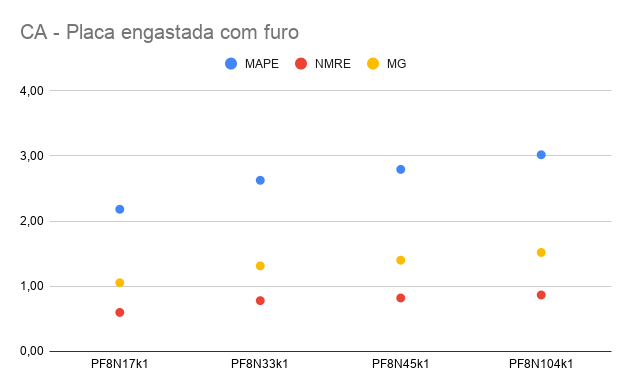
\includegraphics[width=\textwidth]{figuras/Capítulo 5/Placa com furo/CA - Placa engastada com furo.png}
    \label{fig:5.10}
    \centerline{    {\small \textbf{Fonte:} Elaborado pelo autor (2026).}}

\end{figure}


\indent Estudando o CA, é possível chegar às seguintes conclusões: os erros obtidos pelo MEV são inferiores aos obtidos pelo MEF e o MEFG. Para a malha de 208 elementos, o ganho de precisão chega a 1,5 vezes o MEFG. Para a malha mais grosseira o ganho de acurácia é pequeno, sendo equivalente ao MEFG. \\
\indent Como considerações finais desse problema, ressalta-se que, mesmo em problemas com geometrias complexas, a presença de regiões com descontinuidade afeta a aproximação com o método dos elementos virtuais. Algumas soluções são a utilização de métodos de partição da unidade junto ao método dos elementos virtuais, a aplicação de formulações livres de estabilização ou a adoção da formulação para elementos com arestas curvas.

\section{Barragem de terra}

\indent O segundo problema a ser estudado é uma barragem de terra modelada pelo estado plano de deformações, Figura~\ref{fig:5.11}. O modelo de cálculo é um triângulo isósceles sólido com módulo de elasticidade $E = 5,602 \times 10^8\text{ (N/m}^2\text{)}$, densidade $\rho = 2080\text{ (kg/m}^3\text{)}$ e coeficiente de Poisson $\nu = 0,45$.

\begin{figure}[H]
    \centering
    \caption{Geometria da barragem de terra em estado plano de deformações.}
    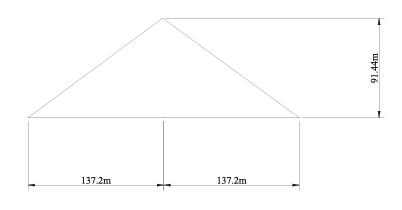
\includegraphics[width=\textwidth]{figuras/Capítulo 5/Barragem/Captura de tela 2026-08-19 082612.png}
    \label{fig:5.11}
    \centerline{    {\small \textbf{Fonte:} Elaborado pelo autor (2026).}}

\end{figure}

\indent O problema de vibrações em barragens de terra foi proposto pela primeira vez por \citet{earthquakestressanalysisearthdams1966}, Figura~\ref{fig:5.12}, como uma extensão dinâmica para a análise de terremotos em barragens de terra. O mesmo problema foi abordado por \citet{analytictrapezoidalfourierpelementvibratingplaneproblems2004} com a utilização de elementos-p Fourier trapezoidais em problemas de vibração no plano, Figura~\ref{fig:5.13}, por \citet{refinednonconformingplanequadrilateralelement2000} no desenvolvimento de um elemento quadrilateral plano não conforme refinado, Figura~\ref{fig:5.14}, e por \citet{cittadin2020enriquecimento} na análise do coeficiente de Friberg junto ao método dos elementos finitos generalizados.

\begin{figure}[H]
    \centering
    \caption{Malha e geometria proposta originalmente.}
    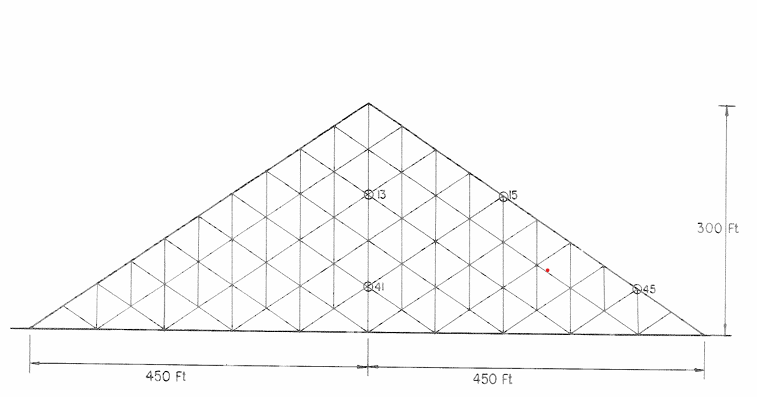
\includegraphics[width=\textwidth]{figuras/Capítulo 5/Barragem/Captura de tela 2026-08-19 083021.png}
    \label{fig:5.12}
    \centerline{    {\small \textbf{Fonte:} \citet{earthquakestressanalysisearthdams1966}.}}

\end{figure}

\begin{figure}[H]
    \centering
    \caption{Discretização por elementos-p Fourier trapezoidais.}
    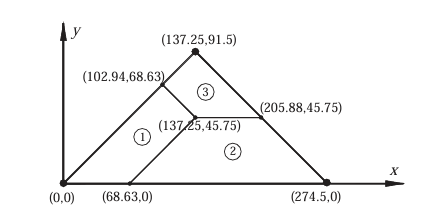
\includegraphics[width=\textwidth]{figuras/Capítulo 5/Barragem/Captura de tela 2026-08-19 082531.png}
    \label{fig:5.13}
    \centerline{    {\small \textbf{Fonte:} \citet{analytictrapezoidalfourierpelementvibratingplaneproblems2004}.}}

\end{figure}

\begin{figure}[H]
    \centering
    \caption{Modelo quadrilateral refinado não conforme.}
    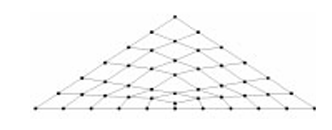
\includegraphics[width=\textwidth]{figuras/Capítulo 5/Barragem/Captura de tela 2026-08-19 082553.png}
    \label{fig:5.14}
    \centerline{    {\small \textbf{Fonte:} \citet{refinednonconformingplanequadrilateralelement2000}.}}

\end{figure}

\indent A primeira análise realizada envolve a malha de 3 elementos de \citet{analytictrapezoidalfourierpelementvibratingplaneproblems2004}. Para o estudo, foram utilizadas inicialmente três malhas de elementos virtuais de 3 elementos cada, contendo 14 g.d.l., 30 g.d.l. e 72 g.d.l. Essas malhas serão utilizadas como forma de comparação com os resultados obtidos pelos demais autores. 

\begin{table}[H]
\caption{Frequências naturais obtidas para a barragem de terra (rad/s).}
\label{tab:5.9}
\begin{tabular}{rllllllll}
\multicolumn{1}{l}{\textbf{MODO}} &
  {[}16{]} (110g.l) &
  {[}17{]} (25g.l) &
  {[}18{]} (72g.l) &
  {[}3{]} MEF (25g.l) &
  {[}3{]} MEFG (182g.l) &
  BT3N7k1 (14g.l) &
  BT3N15k1 (30g.l) &
  BT3N36k1 (72g.l) \\
1 & 7,71  & 7,79  & 7,76  & 7,95  & 7,76  & 7,93   & 7,748  & 7,796  \\
2 & 12,52 & 12,52 & 12,52 & 17,71 & 12,46 & 11,195 & 10,398 & 10,468 \\
3 & 14,6  & 14,51 & 14,49 & 23,44 & 14,34 & 12,041 & 10,614 & 10,629 \\
4 & 19,31 & 18,42 & 18,36 & 30,70 & 18,36 & 15,555 & 10,759 & 10,649
\end{tabular}
\centerline{{\small \textbf{Fonte:} Elaborado pelo autor (2026).}}

\end{table}

\indent Ponderando sobre os efeitos, a primeira frequência apresenta um valor semelhante a todos os autores, contudo, a partir da segunda frequência, os resultados do método dos elementos virtuais tornam-se inferiores aos demais. Utilizando os resultados de \citet{analytictrapezoidalfourierpelementvibratingplaneproblems2004} como referência, calcularam-se os erros obtidos pelo método dos elementos virtuais:

\begin{table}[H]
\caption{Erros relativos (\%) para as malhas de 3 elementos da barragem de terra.}
\label{tab:5.10}
\begin{tabular}{rlll}
\multicolumn{1}{l}{MODO} & BT3N7k1 & BT3N15k1 & BT3N36k1 \\
1                        & 2,85\%  & 0,49\%   & 1,12\%   \\
2                        & 10,58\% & 16,95\%  & 16,39\%  \\
3                        & 17,02\% & 26,85\%  & 26,75\%  \\
4                        & 15,55\% & 41,59\%  & 42,19\% 
\end{tabular}
\centerline{{\small \textbf{Fonte:} Elaborado pelo autor (2026).}}

\end{table}

\begin{figure}[H]
    \centering
    \caption{Erros médios absolutos para cada modo de vibração.}
    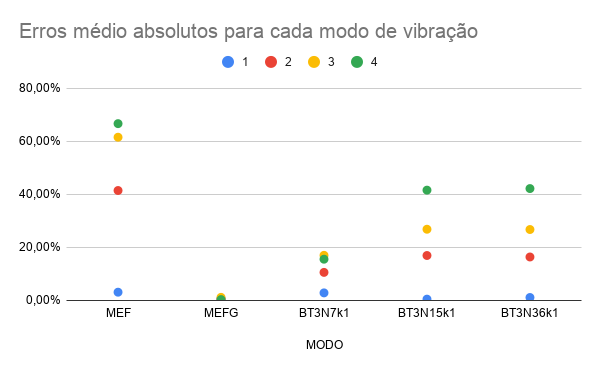
\includegraphics[width=\textwidth]{figuras/Capítulo 5/Barragem/Erros médio absolutos para cada modo de vibração.png}
    \label{fig:5.15}
    \centerline{ {\small \textbf{Fonte:} Elaborado pelo autor (2026).}}
   
\end{figure}


\indent Investigando os erros, percebe-se uma perda de precisão dos resultados para as malhas de 30 g.d.l. e 72 g.d.l. a partir do segundo modo, intensificando-se no quarto modo. Observando o MAPE, nota-se que a malha com 14 graus de liberdade apresenta menor erro do que as malhas de 30 e 72 g.d.l.\\
\indent A aproximação linear permite apenas a representação do campo de deformações constantes por parte da parcela de consistência, com o restante sendo controlado pela parcela de estabilização. Como destacado por \citet{engineeringperspectivevirtualelementmethoditsinterplaystandardfiniteelementmethod2019a}, a função da projeção é garantir que o trabalho virtual interno gerado pelas funções do MEV seja o mesmo provocado pela base polinomial escolhida. Grandes concentrações de nós em uma mesma vizinhança geométrica elástica fazem com que a base de monômios perca sua independência numérica, tornando a matriz $\mathcal{D}$ praticamente linearmente dependente. Como a técnica de estabilização usada neste trabalho utiliza $\mathcal{D}$ em sua construção, derivam-se erros na parcela de estabilização, impondo uma falsa rigidez ao elemento. \citet{illconditioningvirtualelementmethodstabilizationsbases2018} afirma que as diversas técnicas de estabilização presentes na literatura possuem efeitos semelhantes no condicionamento da matriz de rigidez, diferentemente da escolha dos graus de liberdade internos, que possuem impacto profundo.\\
\indent As malhas de 30 g.d.l. e 72 g.d.l. apresentam erros idênticos a partir do segundo modo de vibração. O fenômeno é explicado pela saturação do termo de estabilização. Como detalhado por \citet{basicprinciplesvirtualelementmethods2013a}, a acurácia é ditada pelo grau de interpolação $k$ da projeção polinomial, levando a uma taxa de convergência $O(h^{k+1})$ ótima na norma $L^2$. O aumento do número de arestas não melhora essa taxa teórica se o espaço polinomial se mantiver fixo. Portanto, existe um valor máximo que pode ser assumido pelo termo de consistência e estabilização.\\
\indent Mesmo com os resultados da malha de 3 elementos e 14 g.d.l. obtendo uma resposta melhor que a do método dos elementos finitos com 25 g.d.l., buscou-se obter menores erros nos resultados. Na segunda análise, realizou-se o aumento da quantidade de elementos utilizando a malha de 35 elementos proposta por \citet{refinednonconformingplanequadrilateralelement2000}, e também abordou-se a possibilidade de refino $p$ das malhas, tanto para a malha de 3 elementos quanto para a de 35. 

\begin{table}[H]
\caption{Frequências obtidas com o refino de malha e de ordem polinomial $k=2$.}
\label{tab:5.11}
\begin{tabular}{rllll}
\multicolumn{1}{l}{MODO} & 3BT5N48k1 & BT3N7k2 & BT3N15k2 & BT35N48k2 \\
1                        & 7,768     & 2,038   & 0,000    & 7,723     \\
2                        & 13,598    & 3,164   & 0,000    & 12,642    \\
3                        & 16,809    & 5,665   & 0,000    & 14,964    \\
4                        & 20,785    & 6,816   & 4,251    & 18,789   
\end{tabular}
\centerline{{\small \textbf{Fonte:} Elaborado pelo autor (2026).}}

\end{table}

\begin{table}[H]
\caption{Erros relativos das frequências refinadas e de ordem superior.}
\label{tab:5.12}
\begin{tabular}{rllll}
\multicolumn{1}{l}{MODO} & 3BT5N48k1 & BT3N7k2 & BT3N15k2 & BT35N48k2 \\
1                        & 0,75\%    & 73,57\% & 100,00\% & 0,17\%    \\
2                        & 8,61\%    & 74,73\% & 100,00\% & 0,97\%    \\
3                        & 15,84\%   & 60,96\% & 100,00\% & 3,13\%    \\
4                        & 12,84\%   & 63,00\% & 76,92\%  & 2,00\%   
\end{tabular}
\centerline{{\small \textbf{Fonte:} Elaborado pelo autor (2026).}}

\end{table}

\begin{figure}[H]
    \centering
    \caption{Relação da frequência por modo de vibração para a barragem de terra.}
    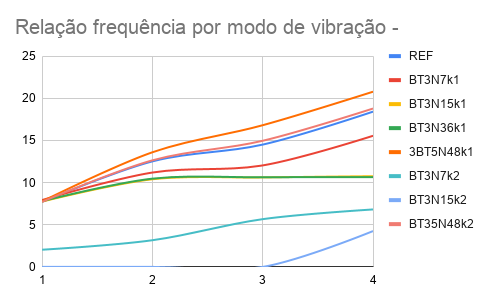
\includegraphics[width=\textwidth]{figuras/Capítulo 5/Barragem/Relação frequência por modo de vibração - Barragem de terra.png}
    \label{fig:5.16}
    \centerline{ {\small \textbf{Fonte:} Elaborado pelo autor (2026).}}
   
\end{figure}

\indent Observando os resultados, percebe-se que as malhas de 35 elementos obtiveram resultados muito próximos da solução de referência, com destaque para a malha de segunda ordem com erro máximo de 3,13\%. Porém, os piores resultados foram os das malhas de 3 elementos de segunda ordem, com a malha 3N15k2 obtendo 100\% de erro.\\
\indent Analisando as frequências da malha 3N15k2, os três primeiros modos foram nulos, o que é um sintoma de modos espúrios de energia. \citet{arbitraryorder2dvirtualelementspolygonalmeshespartelasticproblem2017a} afirma que a função da matriz de estabilização é manter a positividade da forma energética local, e, pela propriedade de estabilidade, a energia elástica computada internamente é equivalente à verdadeira, evitando modos espúrios. Como explicado anteriormente, a norma da forma bilinear é limitada por duas constantes: a constante inferior garante a coercividade e, portanto, a unicidade da solução, enquanto a constante superior garante a continuidade.\\
\indent \citet{virtualelementmethodgeneralsecondorderellipticproblemspolygonalmeshes2016} sustenta que o termo de estabilidade deve ser definido positivo no kernel do projetor $\Pi^\nabla$, garantindo que os únicos modos de energia nula da matriz de rigidez local sejam os movimentos de corpo rígido. A má calibração da matriz de estabilização faz com que o limite inferior tenda a zero, o que implica a perda da capacidade de imposição de resistência elástica às deformações virtuais pertencentes ao $\ker(\Pi_k^\nabla)$ por parte da estabilização, fazendo com que o modelo perca a elipticidade. A malha 3N15k2 ter seus três primeiros modos nulos é, portanto, um indicador de que a matriz de estabilização perdeu a coercividade.\\
\indent Como notado por \citet{illconditioningvirtualelementmethodstabilizationsbases2018}, a dimensão das componentes é dada por:

\begin{equation}
    \begin{aligned}
        \dim(V_{k,1}(\Omega)) = \dim(\mathbb{P}_{k}(\Omega)) = \frac{(k+1)(k+2)}{2} \\
        \dim(V_{k,2}(\Omega)) = \dim(V_{k}(\Omega)) - \dim(V_{k,1}(\Omega)) = (n_v - 2) k - 1. 
    \end{aligned}
\end{equation}


\indent Assim, nota-se que, com o aumento do grau polinomial, ocorre também um aumento do espaço de solução local. \citet{illconditioningvirtualelementmethodstabilizationsbases2018} também destaca que as constantes $a_*$ e $a^*$ têm uma forte dependência com o grau de interpolação, propriedade demonstrada por \citet{exponentialconvergencehpvirtualelementmethodpresencecornersingularities2018}. Essa propriedade implica que a estabilização é bastante sensível a formulações de alta ordem.\\
\indent \citet{engineeringperspectivevirtualelementmethoditsinterplaystandardfiniteelementmethod2019a} explica que a estabilização deve apenas escalar de maneira apropriada, por exemplo, ter a mesma ordem de magnitude que o termo de consistência independentemente da malha. Malhas grosseiras apresentam elementos com grandes proporções; uma má calibragem do parâmetro de estabilização ou um subdimensionamento em relação à escala física do elemento faz com que a estabilização se torne insignificante em relação ao termo de consistência, o que faz com que o limite inferior tenda a zero. \citet{quantitativestudystabilizationparametervirtualelementmethod2024} afirma que, conforme a malha é refinada, a solução virtual se torna insensível ao parâmetro de estabilização porque os modos artificiais passam a possuir menores componentes na solução exata e, mesmo que sua energia não seja exata, seu impacto na solução não é severo.\\
\indent A falha das malhas grossas de segunda ordem pode ser explicada como a soma dos fenômenos de subdimensionamento do parâmetro de estabilização em relação à parcela de consistência somada à sensibilidade das constantes limites de estabilização ao aumento do grau de interpolação, de modo que a matriz de estabilização perde a coercividade e modos artificiais aparecem.\\
\indent Um efeito interessante a ser notado é o aumento do número de condicionamento durante a transição de um problema de primeira para segunda ordem, Figura~\ref{fig:5.17}. \citet{virtualelementmethodtopologyoptimizationpolygonalmeshesnumericalstudy2016} aponta que formulações de elementos virtuais de alta ordem e insuficiência de estabilização em malhas grosseiras levam a elevados mal-condicionamentos das matrizes do sistema e ao aparecimento de modos cinemáticos irrestritos.

\begin{figure}[H]
    \centering
    \caption{Condicionamento de $K$ para o problema da barragem de terra.}
    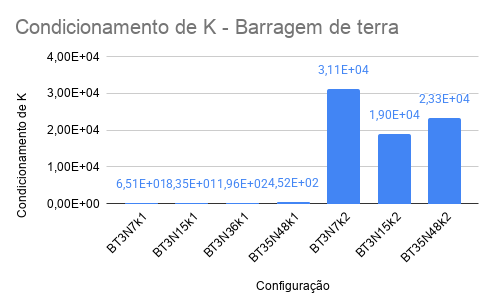
\includegraphics[width=\textwidth]{figuras/Capítulo 5/Barragem/Condicionamento de K - Barragem de terra.png}
    \label{fig:5.17}
    \centerline{{\small \textbf{Fonte:} Elaborado pelo autor (2026).}}
    
\end{figure}

\indent Convertendo os erros absolutos em médias globais, calculam-se o MAPE, NRMSE, MG e o CAD das malhas. Dentre todas as malhas testadas, as únicas que obtiveram CAD positivo foram as de 35 elementos, com a malha de segunda ordem apresentando um ganho de 552\% de eficiência em relação à malha menos refinada.\\
\indent Um ponto a ser notado é: enquanto a malha de segunda ordem com 3 elementos e 30 g.d.l. obteve um erro MAPE de 100\%, para o NRMSE o erro foi de apenas 90,51\%. Esse efeito ocorre porque o quarto modo não foi nulo, afetando o cálculo da média.\\
\indent Mesmo que as malhas 3N72k1 e 35N72k1 possuam a mesma quantidade de graus de liberdade, o CAD da malha de 3 elementos apresenta uma perda de precisão de 581\% em relação à malha mais grossa, em comparação com a malha de 35 elementos que serviu de parâmetro como malha mais refinada, assumindo o valor de 100\%.

\begin{table}[H]
\caption{Métricas globais de erro e coeficiente de acurácia de discretização (CAD) para a barragem de terra.}
\label{tab:5.13}
\begin{tabular}{llllllll}
Métrica & BT3N7k1 & BT3N15k1 & BT3N36k1 & BT35N48k1 & BT3N7k2 & BT3N15k2 & BT35N48k2 \\
MAPE    & 13,07\% & 21,90\%  & 21,57\%  & 10,72\%   & 68,28\% & 100,00\% & 1,49\%    \\
NRMSE   & 14,50\% & 31,99\%  & 32,25\%  & 12,54\%   & 65,89\% & 90,51\%  & 2,16\%    \\
MG      & 13,77\% & 26,47\%  & 26,37\%  & 11,60\%   & 67,08\% & 95,14\%  & 1,79\%    \\
CAD     & 0\%     & -585\%   & -581\%   & 100\%     & -2457\% & -3750\%  & 552\%    
\end{tabular}
\centerline{{\small \textbf{Fonte:} Elaborado pelo autor (2026).}}

\end{table}

\begin{figure}[H]
    \centering
    \caption{Comparação entre as médias dos erros para o problema da barragem de terra.}
    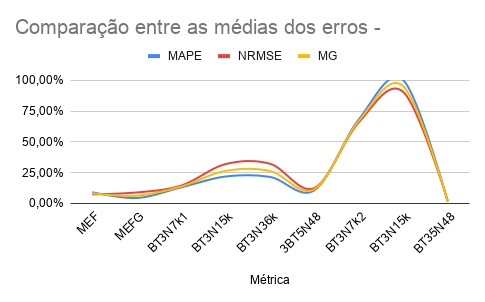
\includegraphics[width=\textwidth]{figuras/Capítulo 5/Barragem/Comparação entre as médias dos erros - Barragem de terra.png}
    \label{fig:5.18}
    \centerline{ {\small \textbf{Fonte:} Elaborado pelo autor (2026).}}
   
\end{figure}


\begin{figure}[H]
    \centering
    \caption{Coeficiente de acurácia de discretização para as malhas da barragem de terra.}
    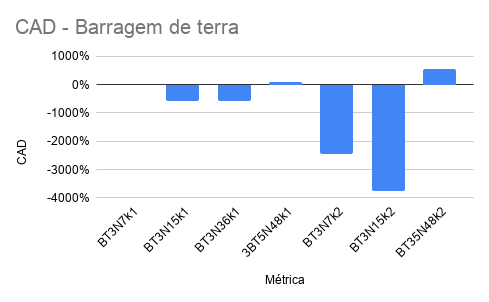
\includegraphics[width=\textwidth]{figuras/Capítulo 5/Barragem/CAD - Barragem de terra.png}
    \label{fig:5.19}
    \centerline{{\small \textbf{Fonte:} Elaborado pelo autor (2026).}}
    
\end{figure}

\indent Para o cálculo do ganho de precisão, serão descartadas as malhas que obtiveram modos espúrios, sobrando apenas a malha de primeira ordem com 3 elementos e 14 g.d.l., e as malhas de 35 elementos. Para comparação entre o método dos elementos virtuais e o método dos elementos finitos generalizados, foram utilizados os valores obtidos por \citet{cittadin2020enriquecimento} para a malha de 35 elementos, a primeira com 94 g.d.l. e a segunda com 1862 g.d.l.

\begin{table}[H]
\caption{Comparação de frequências entre MEF, MEFG e MEV.}
\label{tab:5.14}
\begin{tabular}{rrrrrrr}
\multicolumn{1}{l}{MODO} &
  \multicolumn{1}{c}{REF} &
  \multicolumn{1}{c}{MEF} &
  \multicolumn{1}{c}{MEFG} &
  \multicolumn{1}{l}{BT3N7k1} &
  \multicolumn{1}{l}{3BT5N48k1} &
  \multicolumn{1}{l}{BT35N48k2} \\
1 & 7,71  & 7,797     & 7,7622    & 7,93   & 7,768  & 7,723  \\
4 & 19,31 & 20,859999 & 18,322719 & 15,555 & 20,785 & 18,789
\end{tabular}
\centerline{{\small \textbf{Fonte:} Elaborado pelo autor (2026).}}

\end{table}

\begin{figure}[H]
    \centering
    \caption{Comparação de erros entre os métodos numéricos.}
    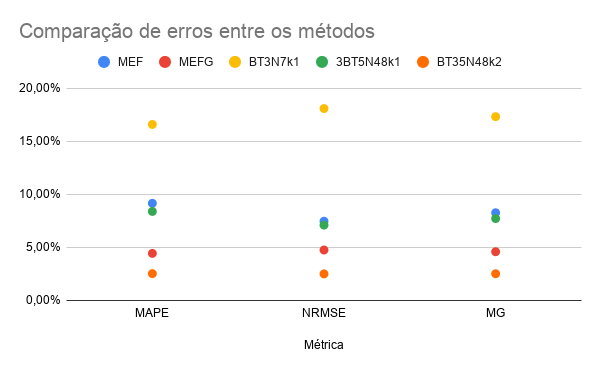
\includegraphics[width=\textwidth]{figuras/Capítulo 5/Barragem/Comparação de erros entre os métodos.png}
    \label{fig:5.20}
    \centerline{    {\small \textbf{Fonte:} Elaborado pelo autor (2026).}}

\end{figure}


\indent Para o primeiro modo de vibração, todos os métodos obtiveram erros menores que 5\%. A diferença entre eles aumenta no quarto modo de vibração, no qual as malhas de elementos virtuais atingem 15,55\% de erro para a malha de 3 elementos e 12,84\% para a malha de 35 elementos. Um resultado interessante a ser observado é que a malha de segunda ordem com 35 elementos e 252 g.d.l. possui os menores erros MAPE entre todos os métodos comparados, superando principalmente o método dos elementos finitos generalizados com 1862 g.d.l.\\
\indent O ganho de precisão das malhas está sumarizado na Tabela~\ref{tab:5.15}. Dentre os resultados, a única malha que conseguiu ter precisão maior que a de elementos finitos foi a malha de segunda ordem com 35 elementos, confirmando a análise de erros.

\begin{table}[H]
\caption{Métricas de erro médio global e comparação com MEF e MEFG.}
\label{tab:5.15}
\begin{tabular}{llllll}
Métrica & MEF    & MEFG   & BT3N7k1 & BT35N48k1 & BT35N48k2 \\
MAPE    & 9,16\% & 4,44\% & 16,59\% & 8,39\%    & 2,53\%    \\
NRMSE   & 7,47\% & 4,75\% & 18,09\% & 7,10\%    & 2,51\%    \\
MG      & 8,27\% & 4,59\% & 17,33\% & 7,72\%    & 2,52\%   
\end{tabular}
\centerline{{\small \textbf{Fonte:} Elaborado pelo autor (2026).}}
\end{table}

\indent Em relação ao CA, a malha de 3 elementos possui valores inferiores tanto ao MEF e precisão de menos 2,5 vezes quando comparada ao MEFG. Em contrapartida, ambas as malhas equilibradas obtiveram erros inferiores ao MEF, entretanto apenas a malha quadrática obteve solução superior ao MEFG, superando a acurácia em uma vez e meia.

\begin{table}[H]
\centering
\caption{CA da barragem de terra}
\label{tab:5.16}
\begin{tabular}{lrrr}
\textbf{Métrica} & \multicolumn{1}{l}{BT3N7k1}   & \multicolumn{1}{l}{3BT5N48k1} & \multicolumn{1}{l}{BT35N48k2} \\
MAPE  & -1,58 & 0,33 & 1,71 \\
NRMSE & -3,92 & 0,18 & 1,42 \\
MG               & \cellcolor[HTML]{D9D9D9}-2,46 & \cellcolor[HTML]{D9D9D9}0,25  & \cellcolor[HTML]{D9D9D9}1,54 
\end{tabular}
\centerline{ {\small \textbf{Fonte:} Elaborado pelo autor (2026).}}
\end{table}


\begin{figure}[H]
    \centering
    \caption{Coeficiente de acurácia relativo da barragem de terra.}
    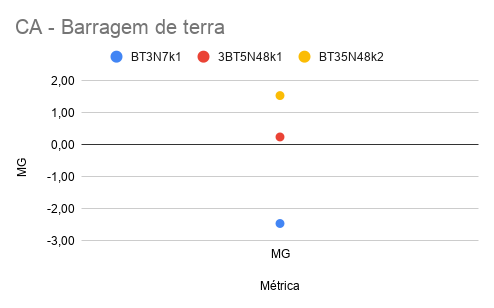
\includegraphics[width=\textwidth]{figuras/Capítulo 5/Barragem/CA - Barragem de terra.png}
    \label{fig:5.21}
    \centerline{{\small \textbf{Fonte:} Elaborado pelo autor (2026).}}
\end{figure}

\section{Parede estrutural}

\indent O terceiro problema abordado consiste em uma parede estrutural no estado plano de tensões, Figura~\ref{fig:5.23}. A parede possui módulo de elasticidade $E = 1\text{ (N/m}^2\text{)}$, massa específica $\rho = 1\text{ (kg/m}^3\text{)}$ e $\nu = 0,2$. 
O problema foi proposto em \citet{nguyenthanh2010alternative} como benchmark para uma formulação alternativa do Método dos Elementos Finitos $\alpha$ (A~$\alpha$~FEM). Os autores comparam a solução com elementos finitos triangulares padrão, uma solução via software ABAQUS, o método dos elementos de contorno e o método sem malha de Petrov-Galerkin local. 

\begin{figure}[H]
    \centering
    \caption{Geometria e modelo da parede estrutural.}
    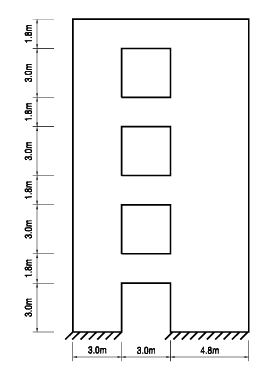
\includegraphics[width=0.5\textwidth]{figuras/Capítulo 5/Parede estrutural/sheer wall.png}
    \label{fig:5.23}
    \centerline{    {\small \textbf{Fonte:} Elaborado pelo autor (2026).}}

\end{figure}

\indent O mesmo problema foi abordado por \citet{custodio2022metodo} com a utilização do MEFG enriquecido com funções trigonométricas. O autor apresenta a comparação entre um elemento enriquecido completo e um elemento enriquecido apenas com funções do tipo bolha. O autor utiliza como referência o A~$\alpha$~FEM de \citet{nguyenthanh2010alternative} e duas famílias de elementos triangulares do MEF, a primeira com aproximação linear e a segunda quadrática.
Para a investigação do problema, serão utilizados apenas elementos triangulares uniformes. Inicialmente, elaboram-se quatro diferentes malhas com todos os elementos triangulares: PE40N48k1, PE112N66k1, PE360N262k1 e PE1000N588k1, Figura~\ref{fig:5.24}. Nota-se que, diferentemente dos problemas anteriores, o aumento da quantidade de elementos é muito maior do que a quantidade de nós ao refinar a malha. \\


\begin{figure}[H]
    \centering
    \caption{Discretizações triangulares para o problema da parede estrutural.}
    \label{fig:5.24}
    \begin{subfigure}[b]{0.45\textwidth}
        \centering
        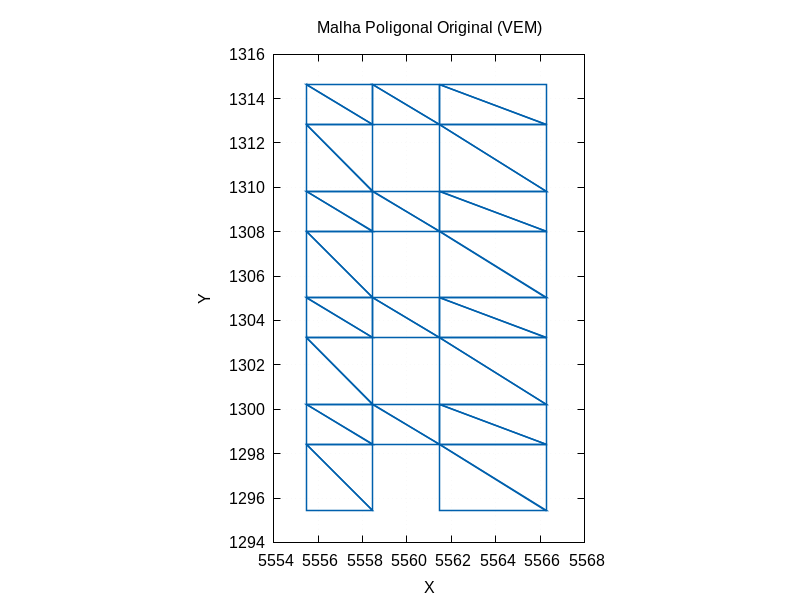
\includegraphics[width=\textwidth]{figuras/Capítulo 5/Parede estrutural/mesh_original 40.png}
        \label{fig:5.24a}
    \end{subfigure}
    \hfill
    \begin{subfigure}[b]{0.45\textwidth}
        \centering
        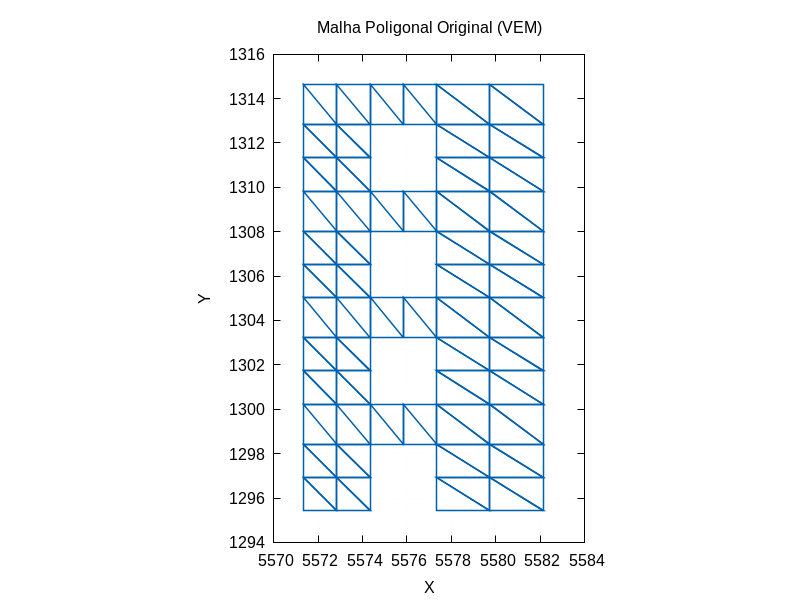
\includegraphics[width=\textwidth]{figuras/Capítulo 5/Parede estrutural/mesh_original 112.png}
        \label{fig:5.24b}
    \end{subfigure}
    \vspace{3mm}
    \begin{subfigure}[b]{0.45\textwidth}
        \centering
        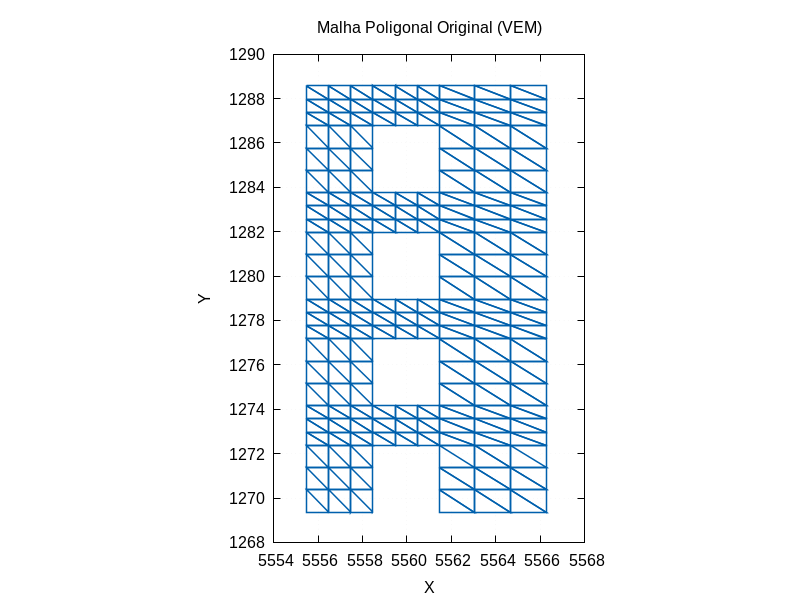
\includegraphics[width=\textwidth]{figuras/Capítulo 5/Parede estrutural/mesh_original 360.png}
        \label{fig:5.24c}
    \end{subfigure}
    \hfill
    \begin{subfigure}[b]{0.45\textwidth}
        \centering
        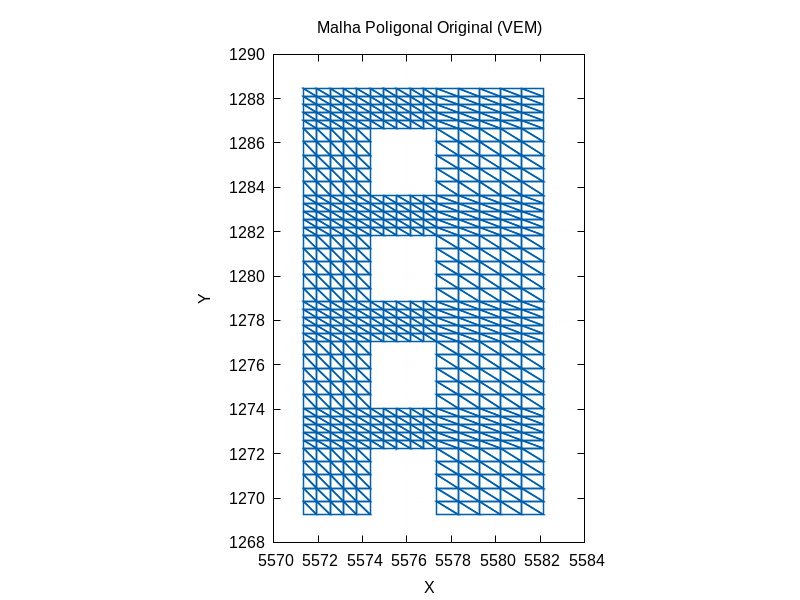
\includegraphics[width=\textwidth]{figuras/Capítulo 5/Parede estrutural/mesh_original 1000.png}
        \label{fig:5.24d}
    \end{subfigure}
    \centerline{    {\small \textbf{Fonte:} Elaborado pelo autor (2026).}}

\end{figure}  



\indent Para o cálculo do erro, como não há solução analítica, utiliza-se o A~$\alpha$~FEM de \citet{nguyenthanh2010alternative} para a obtenção dos erros. Na Figura~\ref{fig:5.25}, observa-se que as frequências obtidas pelo solver de elementos virtuais estão muito acima das frequências de referência, com erros da média geométrica acima de 105\%, o que levou a uma investigação mais profunda das razões.


\begin{table}[H]
\caption{Comparação das frequências de referência com as obtidas através das malhas triangulares de ordem 1.}
\label{tab:5.17}
\begin{tabular}{rlllll}
\multicolumn{1}{l}{Modo} & REF    & PE40N48k1 & PE112N86k1 & PE360N262k1 & PE1000N588k1 \\
1                        & 2,015  & 5,986     & 6,943      & 5,663       & 5,490       \\
2                        & 6,995  & 8,061     & 8,232      & 8,017       & 8,001      \\
3                        & 7,601  & 18,836    & 19,248     & 17,647      & 17,464     \\
4                        & 11,477 & 24,089    & 23,615     & 23,701      & 23,629     \\
5                        & 14,979 & 29,549    & 27,812     & 28,049      & 27,557     \\
6                        & 18,081 & 35,433    & 34,087     & 32,883      & 32,558     \\
7                        & 19,595 & 40,392    & 36,169     & 39,134      & 38,935     \\
8                        & 21,883 & 45,206    & 39,463     & 41,223      & 40,469    
\end{tabular}
\centerline{}
{\small \textbf{Fonte:} Elaborado pelo autor (2026).}
\end{table}


\begin{figure}[H]
    \centering
    \caption{Relação de frequências por modo de vibração para a parede estrutural.}
    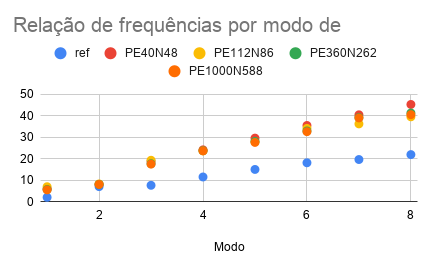
\includegraphics[width=\textwidth]{figuras/Capítulo 5/Parede estrutural/Relação de frequências por modo de vibração.png}
    \label{fig:5.25}
    \centerline{    {\small \textbf{Fonte:} Elaborado pelo autor (2026).}}

\end{figure} 

\begin{table}[H]
\caption{Erros das malhas para elementos virtuais triangulares de primeira ordem na parede estrutural.}
\label{tab:5.18}
\begin{tabular}{lrllll}
Métrica & \multicolumn{1}{c}{MEF} & PE40N48k1  & PE112N86k1 & PE360N262k1 & PE1000N588k1 \\
MAPE    & 33,54\%                 & 106,36\%   & 87,10\%    & 94,05\%     & 91,33\%    \\
NRMSE   & 4,39\%                  & 104,01\%   & 89,04\%    & 92,27\%     & 90,12\%    \\
MG      & 12,13\%                 & 105,18\%   & 88,06\%    & 93,15\%     & 90,72\%   
\end{tabular}
\centerline{{\small \textbf{Fonte:} Elaborado pelo autor (2026).}}

\end{table}

\indent Para verificar o erro, analisam-se os números de condicionamento da matriz de rigidez e verificam-se os mapas de tensões de cisalhamento e de von Mises. \\
\indent Investigando os condicionamentos, Figura~\ref{fig:5.26}, percebe-se que todas as malhas possuem condicionamento acima de $10^6$. Valores de condicionamento altos para malhas de primeira ordem acionam um alerta. Assim, prossegue-se a investigação analisando os mapas de tensões.


\begin{figure}[H]
    \centering
    \caption{Condicionamento da matriz $K$ para as malhas triangulares de primeira ordem.}
    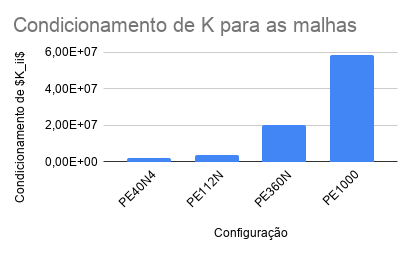
\includegraphics[width=\textwidth]{figuras/Capítulo 5/Parede estrutural/Condicionamento de K para as malhas triangulares.png}
    \label{fig:5.26}
    \centerline{    {\small \textbf{Fonte:} Elaborado pelo autor (2026).}}

\end{figure}


\indent Para análise e dimensionamento de estruturas, existem critérios que indicam a falha do sólido, dentre eles a tensão de von Mises. A tensão de von Mises, ou tensão efetiva, trata-se de um escalar que relaciona as componentes do tensor de tensões. Segundo \citet{elasticitytheoryapplicationsnumerics2021}, se em algum ponto a tensão de von Mises for igual à tensão de escoamento, então o material é considerado estar sob condição de falha. A tensão de von Mises, para o estado plano de tensões, é calculada por: 

\begin{equation}
    \sigma_{\text{vm}} = \sqrt{ (\sigma_{11})^2 - \sigma_{11}\sigma_{22} + (\sigma_{22})^2 + 3(\sigma_{12})^2 }
\end{equation}

\indent O mapa de tensões de von Mises, Figura~\ref{fig:5.27}, apresenta bruscas mudanças no gradiente de tensões, e regiões que deveriam estar sob flexão, como as vigas entre as esquadrias, estão representadas por cores frias. Já para o mapa de tensões de cisalhamento, nota-se um padrão \textit{checkerboard}. Como notado por \citet{checkerboardpatternslayoutoptimization1995}, esse padrão está relacionado com instabilidades numéricas. Isso confirma a hipótese de que o solver está sofrendo travamento por cisalhamento.

\begin{figure}[H]
    \centering
    \caption{Mapa de tensões de von Mises ($k=1$).}
    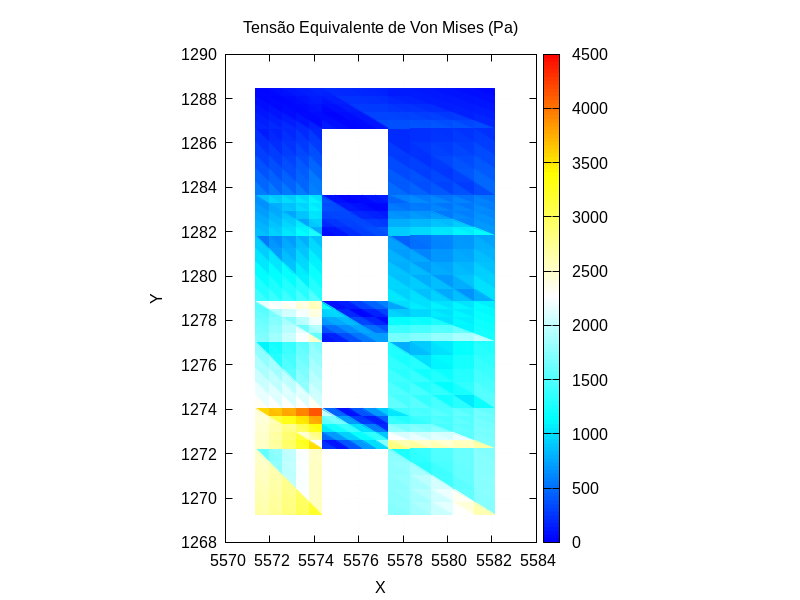
\includegraphics[width=\textwidth]{figuras/Capítulo 5/Parede estrutural/von_mises_map (k1).png}
    \label{fig:5.27}
    \centerline{    {\small \textbf{Fonte:} Elaborado pelo autor (2026).}}

\end{figure}

\begin{figure}[H]
    \centering
    \caption{Mapa de tensões de cisalhamento $\tau_{xy}$ ($k=1$).}
    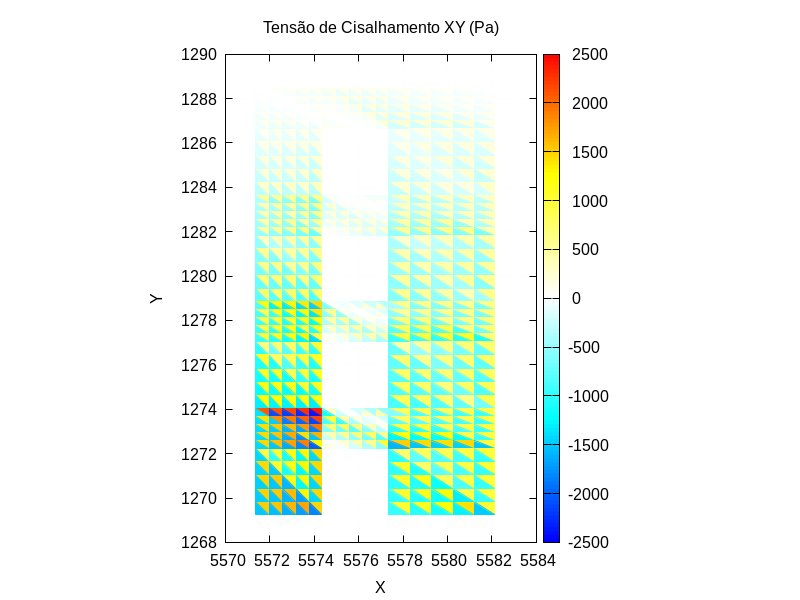
\includegraphics[width=\textwidth]{figuras/Capítulo 5/Parede estrutural/tau_xy_map (k1).png}
    \label{fig:5.28}
    \centerline{    {\small \textbf{Fonte:} Elaborado pelo autor (2026).}}

\end{figure}

\indent A primeira hipótese testada foi que o erro estava sendo causado por conta da aproximação polinomial. Assim, criaram-se as malhas PE40N48k2, PE112N66k2, PE360N262k2 e PE1000N588k2. Essas malhas apresentam a mesma quantidade de elementos que suas contrapartes de ordem 1, mas com a adição dos nós de aresta e do momento interno característicos de formulações de elementos virtuais de segunda ordem. Dos resultados encontrados na Tabela~\ref{tab:5.18}, calculam-se os erros na Tabela~\ref{tab:5.19}, verificando-se que houve uma grande queda do erro em relação à aproximação linear. \citet{virtualelementmethodwheelrailcontactproblems2021} argumenta que grandes espaços de funções virtuais permitem a captura de oscilações, e sua projeção polinomial em espaços polinomiais menores efetivamente os amortece.

\begin{table}[H]
\caption{Frequências para malhas de segunda ordem na parede estrutural.}
\label{tab:5.19}
\begin{tabular}{rlll}
\multicolumn{1}{l}{Modo} & PE40N48k2 & PE112N86k2 & PE360N262k2 \\
1                        & 2,849     & 2,521      & 2,470       \\
2                        & 7,753     & 7,703      & 7,670       \\
3                        & 12,212    & 9,385      & 9,118       \\
4                        & 20,365    & 16,827     & 15,899      \\
5                        & 22,856    & 19,904     & 19,569      \\
6                        & 23,824    & 21,429     & 20,769      \\
7                        & 26,348    & 22,487     & 21,872      \\
8                        & 27,266    & 23,962     & 23,725     
\end{tabular}
\centerline{{\small \textbf{Fonte:} Elaborado pelo autor (2026).}}

\end{table}

\begin{table}[H]
\caption{Métricas de erro para as malhas quadráticas na parede estrutural.}
\label{tab:5.20}
\begin{tabular}{llll}
Métrica & PE40N48k2 & PE112N86k2 & PE360N262k2 \\
MAPE    & 37,93\%   & 20,99\%    & 17,41\%     \\
NRMSE   & 40,46\%   & 22,07\%    & 18,93\%     \\
MG      & 39,17\%   & 21,53\%    & 18,16\%    
\end{tabular}
\centerline{{\small \textbf{Fonte:} Elaborado pelo autor (2026).}}

\end{table}

\indent Mesmo com a queda exponencial do erro, os valores obtidos ainda estavam altos. Assim, testou-se a segunda hipótese de que poderia ser um efeito colateral do parâmetro de estabilização utilizado. Portanto, testa-se a utilização do parâmetro de estabilização proposto por \citet{antonietti2020virtual}: 

\begin{equation}
    \begin{aligned}
        \tau_m = \rho h_E^2 \\
        \tau_k = \max(2\mu , \lambda).
    \end{aligned}
\end{equation}

onde $\mu$ e $\lambda$ são os parâmetros de Lamé.

\indent Substituindo o parâmetro de estabilização, chega-se aos erros com relação às frequências de referência apresentados na Tabela~\ref{tab:5.20}. A primeira observação é que houve uma diminuição do erro, demonstrando a influência do parâmetro de estabilização. Todavia, o erro ainda permanece na casa das dezenas.

\begin{table}[H]
\caption{Erros obtidos com o novo parâmetro de estabilização de Antonietti et al.}
\label{tab:5.21}
\begin{tabular}{llll}
Métrica & PE40N48k2 & PE112N66k2 & PE360N262k2 \\
MAPE    & 16,90\%   & 13,03\%    & 12,59\%     \\
NRMSE   & 16,17\%   & 15,60\%    & 15,19\%     \\
MG      & 16,53\%   & 14,26\%    & 13,83\%    
\end{tabular}
\centerline{{\small \textbf{Fonte:} Elaborado pelo autor (2026).}}

\end{table}


\indent Avaliando os erros obtidos, algumas possibilidades podem ser elencadas para o motivo dos valores elevados mesmo para a formulação quadrática. \citet{numericalrecipeselastodynamicvirtualelementmethodsexplicittimeintegration2020} comenta que a presença de formas de estabilização pode introduzir modos próprios adicionais. Esses modos adicionais pertencem a duas famílias, uma relacionada ao termo de rigidez e outra relacionada ao termo de massa, de maneira inversamente proporcional. O aumento da estabilização de rigidez transfere os modos espúrios para a parte superior do espectro, enquanto a massa transmite esses modos para a parte inferior. \\
\indent Essa relação da massa com a rigidez pode ser observada comparando as curvas de erros de \citet{antonietti2020virtual} e \citet{numericalrecipeselastodynamicvirtualelementmethodsexplicittimeintegration2020}, Figura~\ref{fig:5.29}. O termo de massa utilizado por \citet{numericalrecipeselastodynamicvirtualelementmethodsexplicittimeintegration2020} é baseado na área do elemento e escalonado por ela, enquanto o termo de \citet{antonietti2020virtual} faz o escalonamento pelo diâmetro. O termo de massa tende a deslocar os modos artificiais para as frequências inferiores, enquanto o termo de rigidez tende a deslocar os erros para os termos superiores. O termo de estabilização de massa de \citet{numericalrecipeselastodynamicvirtualelementmethodsexplicittimeintegration2020} tende a ser maior com a redução do tamanho dos elementos por utilizar a área ao quadrado, se comparado ao de \citet{antonietti2020virtual}, ancorando o elemento às frequências mais baixas, o que gera o efeito de translação entre os gráficos. 

    \begin{figure}[H]
        \centering
        \caption{Curvas de erros absolutos com o parâmetro de estabilização de: a) Park et al. e b) Antonietti et al.}
        \label{fig:5.29}
        \begin{subfigure}[b]{0.45\textwidth}
            \centering
            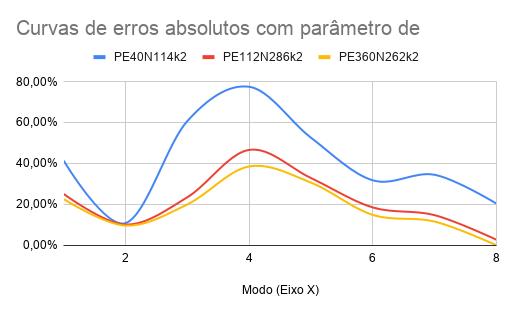
\includegraphics[width=\textwidth]{figuras/Capítulo 5/Parede estrutural/Curvas de erros absolutos com parâmetro de estabilização de Park et al.png}
            \label{fig:5.29a}
        \end{subfigure}
        \hfill
        \begin{subfigure}[b]{0.45\textwidth}
            \centering
            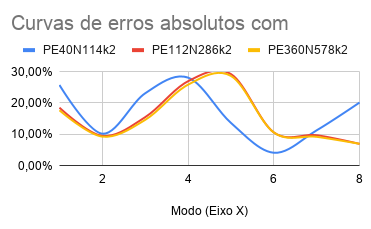
\includegraphics[width=\textwidth]{figuras/Capítulo 5/Parede estrutural/Curvas de erros absolutos com parâmetro de estabilização de Antonietti et al.png}
            \label{fig:5.29b}
        \end{subfigure}
        \centerline{{\small \textbf{Fonte:} Elaborado pelo autor (2026).}}
        
    \end{figure}  

Ao zerar o termo de massa ao mesmo tempo em que se usa a estabilização de rigidez de \citet{antonietti2020virtual}, nota-se uma aproximação das frequências entre a malha mais grossa de 28 elementos e a malha de 360 elementos, ao mesmo tempo em que o impacto na malha de 360 elementos é praticamente nulo, com os erros se originando da rigidez:

\begin{table}[H]
\caption{Frequências calculadas com a anulação da estabilização de massa ($\tau_m=0$).}
\label{tab:5.22}
\begin{tabular}{rrrrr}
\textbf{Modo} & \textbf{REF} & \textbf{PE40N48k2} & \textbf{PE40N48k2 ($\tau_m=0$)} & \textbf{PE360N262k2} \\
1 & 2,015  & 2,534  & \textbf{2,371}  & 2,371  \\
2 & 6,995  & 7,707  & \textbf{7,642}  & 7,642  \\
3 & 7,601  & 9,357  & \textbf{8,713}  & 8,711  \\
4 & 11,477 & 14,703 & \textbf{14,469} & 14,445 \\
5 & 14,979 & 17,022 & \textbf{19,281} & 19,272 \\
6 & 18,081 & 17,341 & \textbf{19,959} & 19,993 \\
7 & 19,595 & 17,387 & \textbf{21,408} & 21,395 \\
8 & 21,883 & 17,473 & \textbf{23,419} & 23,404 \\
\end{tabular}
\centerline{{\small \textbf{Fonte:} Elaborado pelo autor (2026).}}

\end{table}

\indent Esse resultado está de acordo com as conclusões de \citet{boffi2026virtual}, que provam que em problemas de autovalores autoadjuntos elípticos a parcela de estabilização da massa pode ser desconsiderada para formulações padrões de baixa e alta ordem.\\
\indent Como asseverado por \citet{illconditioningvirtualelementmethodstabilizationsbases2018}, os graus de liberdade internos possuem um peso muito maior no condicionamento da matriz de rigidez do que as diversas estabilizações, expondo que os monômios escalados utilizados tradicionalmente na literatura implicam em um aumento exponencial do número de condicionamento em termos de $k$. Fato que pode ser verificado através da Figura~\ref{fig:5.30}. 

\begin{figure}[H]
    \centering
    \caption{Condicionamento da matriz de rigidez após a alteração da estabilização.}
    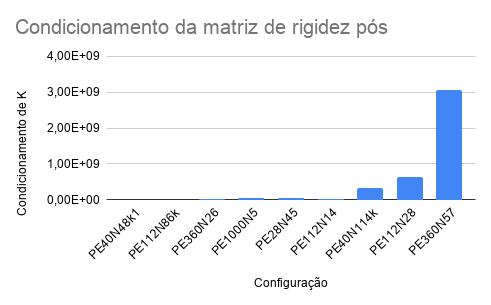
\includegraphics[width=\textwidth]{figuras/Capítulo 5/Parede estrutural/Condicionamento da matriz de rigidez pós mudança de estabilização.png}
    \label{fig:5.30}
    \centerline{    {\small \textbf{Fonte:} Elaborado pelo autor (2026).}}

\end{figure}


\indent Com o aumento do grau polinomial, a base de monômios escalados tende a se tornar colinear. O cálculo das matrizes $\mathcal{G}$ e $\mathcal{H}$ torna-se a solução de sistemas de equações lineares com colunas quase idênticas, o que em aritmética de ponto flutuante causa perda de precisão. Tanto o cálculo do termo de consistência quanto o do termo de estabilização dependem dos operadores de projeção, portanto o aumento da ordem polinomial resulta no surgimento de modos espúrios. \citet{illconditioningvirtualelementmethodstabilizationsbases2018} afirma que uma forma de combater esse efeito é o emprego da base canônica ortonormal, que pode ser construída através do algoritmo de Gram-Schmidt. \\
\indent Outra consideração que deve ser feita é que a estabilização de \citet{numericalrecipeselastodynamicvirtualelementmethodsexplicittimeintegration2020} é escalada com base na parcela de consistência, enquanto a de \citet{antonietti2020virtual} é escalonada puramente nas propriedades elásticas do material. Isso pode explicar parcialmente a redução do erro ao realizar a substituição do parâmetro de estabilização.\\
\indent Para comparação dos resultados, serão tomados os valores do MEF quadrático e do MEFG de \citet{custodio2022metodo}. Os erros entre os métodos e a formulação de referência (A~$\alpha$~FEM) encontram-se na Tabela~\ref{tab:5.22}. Desses resultados, é interessante notar que nem o MEV e nem o MEFG obtiveram respostas melhores que o MEF quadrático.

\begin{table}[H]
\caption{Comparação de erros do MEV com o MEF-T6 e MEFG.}
\label{tab:5.23}
\begin{tabular}{lrrlll}
Métrica & \multicolumn{1}{l}{MEF-T6} & \multicolumn{1}{c}{MEFG} & PE40N48k2 & PE112N66k2 & PE360N262k2 \\
MAPE  & 6,30\% & 11,26\% & 16,90\% & 13,03\% & 12,59\% \\
NRMSE & 1,24\% & 1,26\%  & 16,17\% & 15,60\% & 15,19\% \\
MG    & 2,80\% & 3,77\%  & 16,53\% & 14,26\% & 13,83\%
\end{tabular}
\centerline{{\small \textbf{Fonte:} Elaborado pelo autor (2026).}}

\end{table}



\indent Como nenhum resultado do MEV foi melhor que o do MEF, não há motivo para calcular os valores de ganho de precisão de discretização, mas calcula-se o coeficiente de acurácia. Observando a Tabela~\ref{tab:5.23}, existe a impressão de que os resultados do MEV foram superiores aos resultados do MEFG. Entretanto, os resultados do CAD indicam o quão impreciso foi o MEV. Os resultados positivos ocorrem devido a ambas as técnicas terem sido inferiores ao MEF.

\begin{table}[H]
\caption{Valores do CAD calculados para a parede estrutural.}
\label{tab:5.24}
\begin{tabular}{lrrrrr}
Métrica &
  \multicolumn{1}{l}{PE28N45k2} &
  \multicolumn{1}{l}{PE40N48k2} &
  \multicolumn{1}{l}{PE122N66k2} &
  \multicolumn{1}{l}{PE112N145k2} &
  \multicolumn{1}{l}{PE360N262k2} \\
MAPE  & 1,38   & 2,14   & 1,36   & 1,06   & 1,27   \\
NRMSE & 585,73 & 885,29 & 851,38 & 794,60 & 827,21 \\
MG &
  \cellcolor[HTML]{D9D9D9}9,59 &
  \cellcolor[HTML]{D9D9D9}14,16 &
  \cellcolor[HTML]{D9D9D9}11,82 &
  \cellcolor[HTML]{D9D9D9}10,53 &
  \cellcolor[HTML]{D9D9D9}11,38
\end{tabular}
\centerline{{\small \textbf{Fonte:} Elaborado pelo autor (2026).}}

\end{table}

\indent Para os modos de vibração na malha de 360 elementos de segunda ordem, os modos com menores erros foram o segundo e o oitavo. Os deslocamentos podem ser vistos na Figura~\ref{fig:5.31}.

    \begin{figure}[H]
        \centering
        \caption{Deformações correspondentes ao: a) 2º modo e b) 8º modo de vibração.}
        \label{fig:5.31}
        \begin{subfigure}[b]{0.45\textwidth}
            \centering
            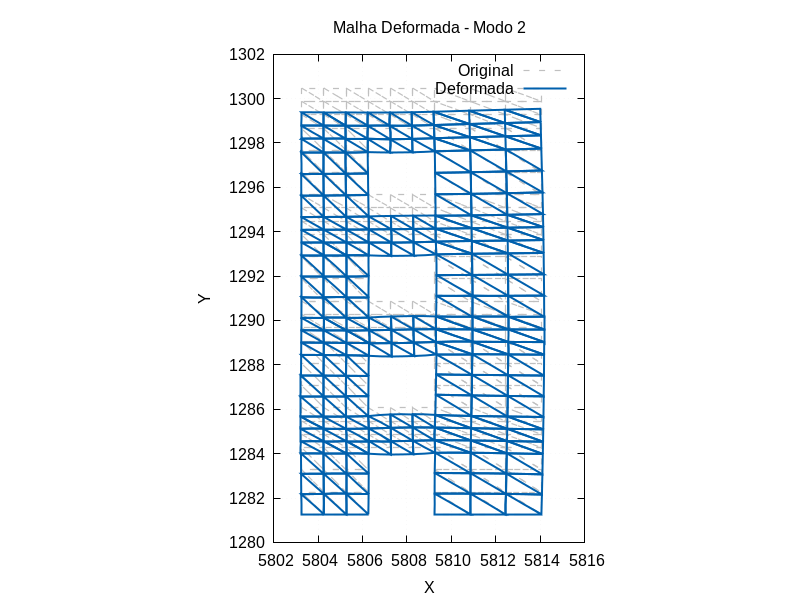
\includegraphics[width=\textwidth]{figuras/Capítulo 5/Parede estrutural/deformed_mode_2.png}
            \label{fig:5.31a}
        \end{subfigure}
        \hfill
        \begin{subfigure}[b]{0.45\textwidth}
            \centering
            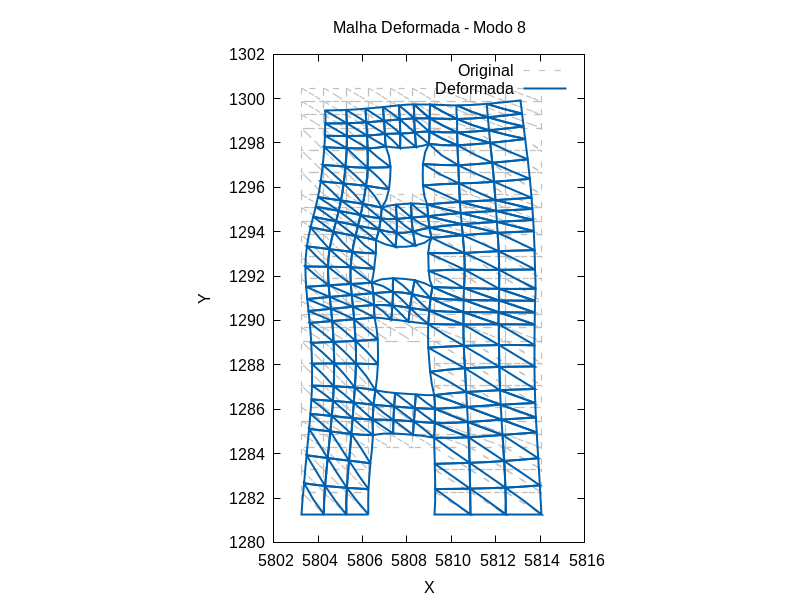
\includegraphics[width=\textwidth]{figuras/Capítulo 5/Parede estrutural/deformed_mode_8.png}
            \label{fig:5.31b}
        \end{subfigure}
        \centerline{        {\small \textbf{Fonte:} Elaborado pelo autor (2026).}}

    \end{figure} 


\indent Em relação ao tempo de execução, nota-se pela Figura~\ref{fig:5.32} que, apesar de a quantidade de elementos estar relacionada ao tempo de processamento, o grau de aproximação possui um impacto muito maior. Nota-se que o tempo de montagem do elemento é muito mais curto do que o tempo de solução do sistema. Da Figura~\ref{fig:5.33}, é possível inferir que o condicionamento apresenta pouco impacto no tempo total de execução do solver, sendo este mais impactado pela quantidade de elementos e pelo grau polinomial.


\begin{figure}[H]
    \centering
    \caption{Tempo de execução em função do número de elementos: a) $k=1$ e b) $k=2$.}
    \label{fig:5.32}
    \begin{subfigure}[b]{0.45\textwidth}
        \centering
        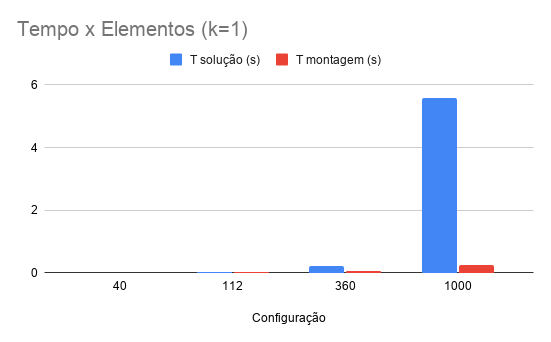
\includegraphics[width=\textwidth]{figuras/Capítulo 5/Parede estrutural/Tempo x Elementos (k=1).png}
        \label{fig:5.32a}
    \end{subfigure}
    \hfill
    \begin{subfigure}[b]{0.45\textwidth}
        \centering
        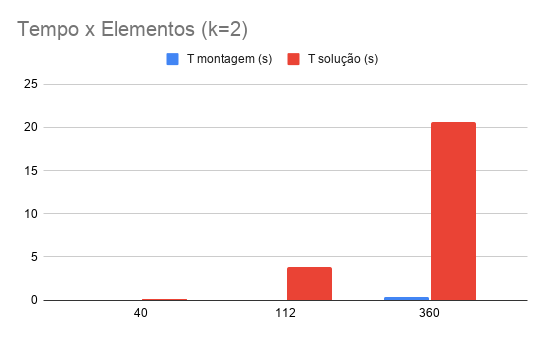
\includegraphics[width=\textwidth]{figuras/Capítulo 5/Parede estrutural/Tempo x Elementos (k=2).png}
        \label{fig:5.32b}
    \end{subfigure}
    \centerline{    {\small \textbf{Fonte:} Elaborado pelo autor (2026).}}

\end{figure} 

\begin{figure}[H]
    \centering
    \caption{Relação entre o número de condicionamento e o tempo de execução.}
    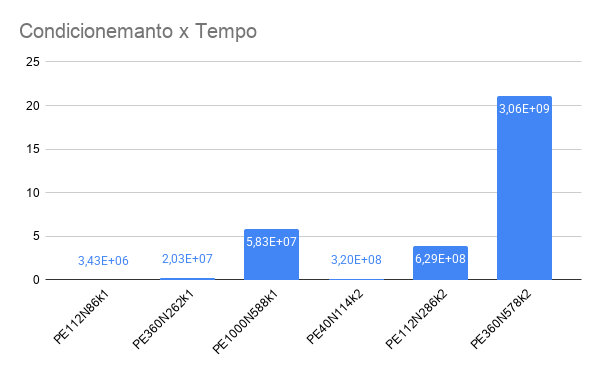
\includegraphics[width=\textwidth]{figuras/Capítulo 5/Parede estrutural/Condicionemanto x Tempo.png}
    \label{fig:5.33}
    \centerline{{\small \textbf{Fonte:} Elaborado pelo autor (2026).}}
\end{figure}